%%%%%%%%%%%%%%%%%%%%%%%%%%%%%%%%%%%%%%%%%%%%%%%%%%%%%%%
% A template for Wiley article submissions.
% Developed by Overleaf. 
%
% Please note that whilst this template provides a 
% preview of the typeset manuscript for submission, it 
% will not necessarily be the final publication layout.
%
% Usage notes:
% The "blind" option will make anonymous all author, affiliation, correspondence and funding information.
% Use "num-refs" option for numerical citation and references style.
% Use "alpha-refs" option for author-year citation and references style.

\documentclass[alpha-refs]{wiley-article-05g}
% \documentclass[blind,num-refs]{wiley-article}

% Add additional packages here if required
\usepackage{siunitx}

% For figures
\usepackage{graphics}

%For captions - even though template has complex caption commands
\usepackage[labelfont=bf,justification=centering]{caption}
\usepackage[font=small,labelfont=bf]{subcaption}
\captionsetup[sub]{font=small,labelfont={bf,sf}}

%% For figures numbered by section
\usepackage{chngcntr}
\counterwithin{figure}{section}
\counterwithin{table}{section}


%% Additional links for hyperref
\usepackage[unicode=true,pdfusetitle,
 bookmarks=true,bookmarksnumbered=true,bookmarksopen=true,bookmarksopenlevel=2,
 breaklinks=false,pdfborder={0 0 1},backref=false,colorlinks=false]
 {hyperref}
\hypersetup{pdfstartview={XYZ null null 1}}


%% For fillers
\usepackage{lipsum}

%% For references 
\usepackage[backend=bibtex,
			natbib=true, 
			style=chicago-authordate]{biblatex}
\addbibresource{Returns.bib}

\usepackage{array}
\usepackage{longtable}
%\usepackage{fullpage}

\usepackage{lmodern}
\newcommand{\graph}[3]{
\raisebox{-#1mm}{\includegraphics[height=#2em,width=3cm]{#3}}
}

\usepackage{booktabs} % for vertically partitioned table

% for  table with itemized list
\usepackage{tabularx}
\usepackage{enumitem}
\newlist{tabitemize}{itemize}{1}
\setlist[tabitemize]{label=\textbullet,leftmargin=*,topsep=0ex,parsep=0pt,
                  after=\vspace{-\baselineskip},before=\vspace{-0.75\baselineskip}}  

%\usepackage{makecell}  % for cell alignment

\usepackage[export]{adjustbox} % for figure in frame


\usepackage{array}
\newcolumntype{L}[1]{>{\raggedright\let\newline\\\arraybackslash\hspace{0pt}}m{#1}}
\newcolumntype{C}[1]{>{\centering\let\newline\\\arraybackslash\hspace{0pt}}m{#1}}
\newcolumntype{R}[1]{>{\raggedleft\let\newline\\\arraybackslash\hspace{0pt}}m{#1}}

%%%%%%%%#################################################################################%%%%%%%%%%%%%%%%%%%%%%%%%%%%%

% Update article type if known
\papertype{WORLD BANK EDUCATION GLOBAL PRACTICE}
% Include section in journal if known, otherwise delete
\paperfield{Russian Federation: Analytical Services and Advisory Activity: 
P170978}

\title{Returns to Education in the Russian Federation: Towards Evidence Based Decision Making with Social and Private Returns to Education}

% List acknowledgements here.
\fundinginfo{Thanks are due to the Ministry of Education for the graduate.ru website that provides data on graduates earnings available to the public. Thanks are due to the Ministry of Finance for the bus.gov.ru website that provides the data on revenues received by all public institutions including colleges and universities. The code used for this paper is made freely available for all researchers at \url{https://bitbucket.org/zagamog/edreru/src/master/}}

% Include full author names and degrees, when required by the journal.
% Use the \authfn to add symbols for additional footnotes and present addresses, if any. Usually start with 1 for notes about author contributions; then continuing with 2 etc if any author has a different present address.

\author[*]{Ekaterina Melianova}
\author[*]{\hspace{-1em}Suhas Parandekar}
\author[*]{\hspace{-1em}Art\"{e}m Volgin}

% List abbreviations here, if any. Please note that it is preferred that abbreviations be defined at the first instance they appear in the text, rather than creating an abbreviations list.
\acks{\begin{normalsize}
\emph{Country Director:} Renaud Seligman; \emph{Regional Director:} Fadia Saadah; \emph{Practice Manager:} Harry Patrinos; \emph{Program Leader:} Dorota Nowak; \emph{Peer Reviewers}: Cristian Aedo; Ruslan Yemtsov; Husein Abdul-Hamid; \emph{Team members:} Polina Zavalina; Zhanna Terlyga. Any errors are a responsibility of the authors.
\end{normalsize}
\vspace{-0.2in}}

%\contrib[\authfn{1}]{Equally contributing authors.}

% Include full affiliation details for all authors
\affil[*]{Education Global Practice, Europe and Central Asia}

%\corraddress{Author One PhD, Department, Institution, City, State or Province, Postal Code, Country}
\corremail{sparandekar@worldbank.org}

%\presentadd[\authfn{2}]{Department, Institution, City, State or Province, Postal Code, Country}

% Include the name of the author that should appear in the running header
\runningauthor{P170978: WP05 - Private and Social Returns to Education}



\begin{document}

\maketitle

\begin{abstract}
\vspace{.5em}
This paper is the fourth and final one in a series of working papers investigating the returns to education in the Russian Federation. This paper uses institution level information about graduate earnings and estimates of social and private costs to obtain social and private returns to education using an internal rates of return calculation. As data has been collected so far only on earnings trajectories for three years following graduation, these are not lifetime returns, but they are adequate to provide relative estimates. Samara Energy College \url{https://sam-ek.ru/} with private returns of 35\% and social returns of 13\%. V. R. Fillipova Buryat State Agricultural Academy in Ulan Ude \url{http://www.bgsha.ru/} leads the universities list with a private returns of 9\% and social return of 7\%. Even though the results presented here are of a preliminary nature, the data length and model sophistication can only grow in the future.The resulting information on returns to investment will serve government stakeholders as well as individual students.  

% Please include a maximum of seven keywords
\keywords{Returns to Education, Russian Federation, Universities, Colleges \emph{JEL Codes: I23, I26}}
\end{abstract}

\section{Data Sources}

This paper provides a practical demonstration of the efficacy of open data 
and the possibility of combining open data from different sources to 
provide valuable information. The data pertain to the return to investment 
in a college or university education, one of the most important decisions 
made by an individual, and collectively of critical importance to Russia's 
future growth and social prosperity. Two different open data sources are 
used for this paper. The data are not officially linked and one of the 
technically challenging but tedious tasks performed by the authors of this 
paper was the merging of two data sets - one from the Ministry of 
Education, and the other from the Ministry of Finance. This paper provides 
a brief overview of the datasets in this section, followed by two sections 
of substantive results. The next section combines earnings data from 
Rosstat's Survey of Income and Social Programs with cost data from the 
Ministry of Finance to provide regional estimates of social and private 
returns to education. To the best of our knowledge, social returns have not 
been published before for the Russian Federation. The third section 
presents data at an institutional level, with returns to education that 
could guide students making decisions to enroll in a college or university. 
The information could also serve public officials to benchmark returns as a 
means to improve systemic efficiency. 

\subsection{Graduate.edu.ru from the Ministry of Education}

\url{Graduate.edu.ru} is the official graduate employment monitoring portal 
created and maintained by the Ministry of Education of the Russian 
Federation. The website was launched in 2015 to provide information 
targeted mainly to prospective graduates about the employment record of 
graduates from tertiary education institutions - including universities and 
vocational education colleges. The official record is contained in Minutes 
No. DL-57, dated December 22, 2014 of the Interdepartmental Commission for 
Monitoring the Efficiency of Higher Education Educational Organizations. It 
is a complex organizational feat to carry out accurate and valid data 
collection of this nature. Figure \ref{fig:1.1} is a translation of an 
infographic that explains the process of data collection. 

\vspace{0.5em}

Rosobrnadzor (Federal Service for Supervision in Education and Science) 
registers graduation certificates from issuing institutions. After 
verification, a request for salary information for the graduates is sent to 
the PFRF (Pension Fund for the Russian Federation).  There is a high degree 
of compliance from educational institutions and the high fidelity in terms 
of obtaining information from graduates. For example, for the year 2014, 
information was provided by 2,841 colleges and 834 universities, which 
tracks quite well with the 2,909 colleges and 950 universities that existed 
in 2014 according to Rosstat, including both public and private 
institutions. The number of graduates in 2014 from Rosstat (just over 1 
million from universities; around half a million graduates for vocational 
education) conforms to the number of Rosobrnadzor records of graduates. 
Interestingly only a minuscule portion of individuals were not able to be 
tracked by the PFRF because of filing errors - 0.78 \% for colleges and 
0.15 \% for universities. Further, in relation to the scale and complexity 
of the task, only a  small number of domestic working graduates were not 
able to be matched with income information from PFRF - 8\% for colleges and 
5\% for universities. In other words, 92\% of college graduates and 95\% of 
university graduates had their salary information recorded in graduate.edu. 

\vspace{0.5em}

To get the maximum possible span from the available data,  we use the information of graduates in 2013 in each university and college and their corresponding salaries in 2014, 2015 and 2016. Our final set of data consists of 1909 colleges, 423 universities, and 2975 pairs of university-study areas with information about the graduates earning in them. We filtered out universities and colleges with less than 100 and 50 graduates in 2013, respectively. Salaries in 2014 and 2015 were adjusted to the prices of 2016. 

\begin{center}
	\begin{figure}[htbp!]
\begin{minipage}[b]{1\linewidth}
			\centering
			\hspace*{-0.2in}
         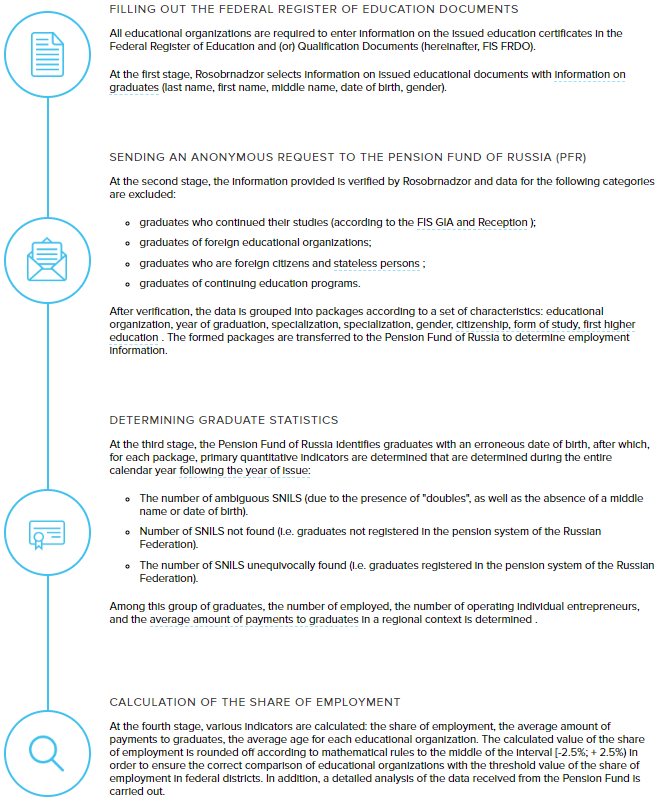
\includegraphics[scale=0.88, frame]{gedu_cap1b.png}
			% plot 1
		\end{minipage}
			\caption{Four step process of data collection - Infographic from graduate.edu.ru}\label{fig:1.1}
	\end{figure}
\end{center}

\vspace{-0.35in}

Table \ref{tab:1.1} provides mean earnings in 2016 rubles, for college and university graduates. These numbers are consistent with the wage earnings information reported in Rosstat's Statistical Survey of Income and Participation in Social Programs. An interesting fact to note from the table is that university graduates just 3 years from graduation earn about 1/3rd more than vocational school graduates; overt the lifecycle this difference tends to grow to 50\% or 60\% more. The purpose of this paper is to compare between private and social costs across regions and institutions. The lower differentials reported in Table \ref{tab:1.1} point to the fact that the returns presented in this paper should not be considered as life-time returns. 

\begin{table}[htbp!]
    \centering
		\caption{Average Earnings reported by graduate.ru}
		\label{tab:1.1}\\
    \begin{tabular}{|l|l|l|l|l|l|}
    \hline
         & Mean & Std & Quantile.25. & Quantile.50. & Quantile.75. \\ \hline
        College Graduates Avg. Earnings 2014 & 301,255 & 81,712 & 247,093 & 279,156 & 328,995 \\ \hline
        College Graduates Avg. Earnings 2015 & 281,567 & 76,821 & 229,697 & 261,667 & 311,208 \\ \hline
        College Graduates Avg. Earnings 2016 & 287,918 & 80,574 & 233,763 & 267,480 & 320,583 \\ \hline
        University Graduates Avg. Earnings 2014 & 411,050 & 152,936 & 300,829 & 365,771 & 481,628 \\ \hline
        University Graduates Avg. Earnings 2015 & 419,488 & 158,256 & 304,798 & 368,518 & 496,961 \\ \hline
        University Graduates Avg. Earnings 2016 & 433,387 & 175,586 & 305,856 & 380,304 & 508,152 \\ \hline
    \end{tabular}
\end{table}

\vspace{-0.3in}

\subsection{Bus.gov.ru from the Ministry of Finance}

The next data source used in this paper is from \url{bus.gov.ru}, the transparency promoting website managed by the Ministry of Finance, with more than 160,000 institutions from many sectors including health and education. 

\vspace{-0.25in}

\begin{center}
	\begin{figure}[htbp!]
\begin{minipage}[b]{1\linewidth}
			\centering
			\hspace*{-0.1in}
         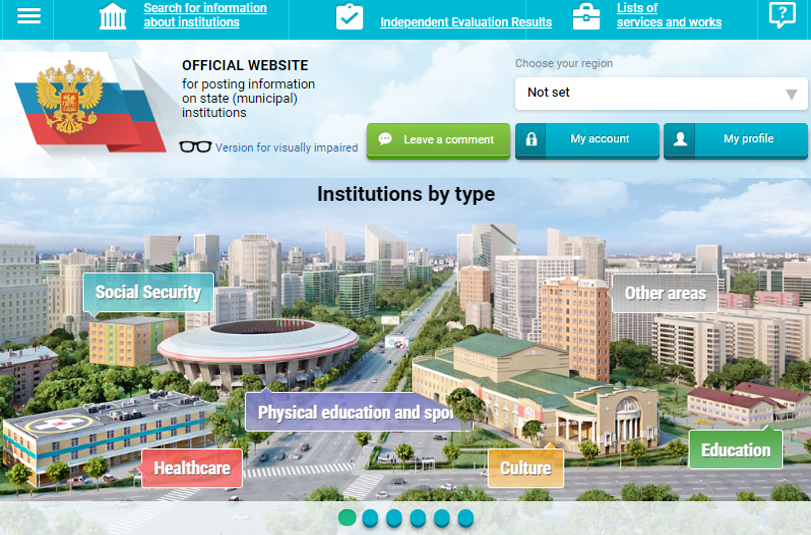
\includegraphics[scale=0.4, width=5.6in, frame]{busg_cap1c.png}
			% plot 1
		\end{minipage}
			\caption{Website for bus.gov.ru}\label{fig:1.2}
	\end{figure}
\end{center}

\vspace{-0.2in}

The bus.gov.ru website is indicated to be the official website of the Russian Federation for provision of information by public institutions, based on Order No. 86n of the Ministry of Finance of the Russian Federation, dated July 21, 2011. The objective as stated on the website is ``to increase the openness and accessibility of information about state (municipal) institutions, as well as about their activities and property''. As with the elaborate process between Rosobrnadzor and PFRF, the bus.gov.ru website appears to be created with great attention to detail. One of the features that makes the site function effectively is the automation of procedures for posting information. Information with significant level of detail is collected at the website, including service quality ratings, financial information and information about the financial capital where relevant. \footnote{Recently, the World Bank published a report looking at a portion of the data from the website - the independent evaluation ratings on 16 service quality dimensions - to compute efficiency measurements of extra-curricular activities, a big expenditure item for the education sector. See \textit{Russian Federation: Doing Extra-Curricular Education: Blending Traditional and Digital Activities for Equitable Learning}}

\vspace{0.5em}

This paper is based on use of the information pertaining to the annual revenues of colleges and universities. Information is available for the total annual revenue from different sources including government transfers and grants, as well as revenue from service payments made by private individuals. For education institutions (colleges and universities) we assume that the revenues from service payments are tuition fee payments.\footnote{This is an approximation in some cases where educational institution charge fees for non-educational services.} Revenue information is used to estimate costs rather than expenditure information because we need to separate between overall costs of an institution, and the portion of costs that are subsidized by the State. Table \ref{tab:1.2} provides a summary of the information from bus.gov.ru used for this paper. 

\begin{table}[htbp!]
    \centering
		\caption{Derivation of College and University costs from bus.gov.ru data}
		\label{tab:1.2}\\
    \begin{tabular}{|p{6cm}|r|r|r|}
    \hline
       \multicolumn{4}{|c|}{\textbf{Colleges}} \\ \hline
       & Mean & Quantile.25. & Quantile.75. \\ \hline
        Total Cash Receipts - mean for 2012-2017 & 106,233,973 & 47,882,033 & 109,940,985 \\ \hline
        Cash Receipts from Paid Services  & 13,423,225 & 4,220,980 & 17,147,603 \\ \hline
        Cash Receipts from Targeted Subsidies  & 13,644,089 & 2,973,843 & 13,122,018 \\ \hline
        Cash Receipts from the Budget Investments  & 380,156 & -  & - \\ \hline
        Cash Receipts from the State (Municipal) Tasks  & 71,886,730 & 34,835,450 & 77,701,603 \\ \hline
        Social Cost per student for Colleges & 206,856 & 110,175 & 248,683 \\ \hline
        Private Cost per student (excludes govt. revenue sources)  & 24,287 & 10,204 & 32,854 \\ \hline
       \multicolumn{4}{|c|}{\textbf{Universities}} \\ \hline
           Total Cash Receipts - mean for 2012-2017 & 1,557,966,861 & 488,137,618 & 1,555,625,338 \\ \hline
        Cash Receipts from Paid Services & 553,941,067 & 133,154,544 & 663,924,931 \\ \hline
        Cash Receipts from Targeted Subsidies  & 219,389,727 & 75,000,342 & 220,372,051 \\ \hline
        Cash Receipts from the Budget Investments  & 35,201,477 & - & 3,125,759 \\ \hline
        Cash Receipts from the State (Municipal) Tasks  & 653,606,278 & 246,276,440 & 649,967,746 \\ \hline
        Social Cost per student for Universities & 264,869 & 107,278 & 308,393 \\ \hline
        Private Cost per student (excludes govt. revenue sources) & 97,452 & 34,450 & 112,030 \\ \hline
    \end{tabular}
\end{table}

\vspace{-0.2in}

\section{Regional Private and Social Returns to Education for the Russian Federation}

\subsection{Background}

The returns to education that are calculated by the classical Mincerian 
equation are private returns that accrue to individuals 
\parencite{mincer1974}. This paper presents the `narrow social returns to 
education' as defined in \cite{psacharopoulos2019}. The classical 
computation implicitly includes only the indirect cost of education. This 
is the opportunity cost to an individual of being in school rather than 
working in the labor market and earning a wage. The standard Mincerian 
formulation does not include the direct costs of education to an individual 
- tuition fees, textbooks and other associated expenditures. The Mincerian 
formulation also does not include the public or social costs incurred in 
the provision of education. The `full-discounting method' of calculating 
returns is the name given to the internal rate of return used to discount 
the future stream of earnings to equal the costs of education 
\parencite{psacharopoulos1995}. When the costs include only the costs 
incurred by individuals, these are private returns to education; when the 
costs also include the public subsidies usually provided for education, 
they are termed as the social return to education. They are termed as the 
'narrow' social returns because they do not include the possible social 
benefits of education due to externalities such as reduced crime, better 
financial decisions and effects on the environment and the innovative 
capabilities of a society, to name a few of the external effects 
\parencite{wolfe2002,mcmahon2004,owens2004}.  The utility of computing the 
narrow social returns of education is to measure the efficiency of public 
spending. \cite{Psacharopoulos_Patrinos2018} present global estimates of 
both private and social returns for a comparison between levels of 
education across countries. In this paper we extend the computation of 
private and social returns within the Russian Federation. 

\subsection{Limitations of the data} 

The computation of social rates of return involve some simplifications that 
constitute a limitation of this paper. With a sample size in excess of 
50,000 individuals, the Rosstat Statistical Survey of Income and 
Participation in Social Programs for 2018 (latest year available) provides 
regionally representative estimates of the age earnings profile for 
individuals. The cost side of the full discounting method comes from the 
regional weighted average costs of institutions within a region. This 
abstracts away from migration of individuals for the purpose of education 
and obtaining a job. Individuals might move away from a region only for the 
purpose of studying in another region and then return to the region for 
work. Typically, this education would take place in Moscow or St. 
Petersburg, where the costs would be higher than the `sending' region. 
However, our method attributes the costs of the sending region as the 
default cost, thus tending to overestimate the returns to education for 
Moscow and St. Petersburg Unobserved abilities or motivation that affects 
migration decisions would further complicate the scenario. There are a 
range of other migration effects. Individuals might migrate to study and 
then settle down in the same region where they study, example in Moscow. In 
this case, there would be no bias in the regional estimates of returns to 
education. Individuals might also study in one region and then migrate only 
for work, and the relative costs of education in the two regions would 
determine the sign of the bias in the estimation of returns.  Future 
improvements of this paper should incorporate the effects of migration to 
estimate more accurate returns to education. 
Another simplification is entailed in the cost calculations used in this paper. There is no ready way to validate the cost figures for colleges and universities as a cost database does not yet exist for the Russian Federation. Instead, we are using revenues of the institutions divided by an approximate measure of the number of students to arrive at an estimate of unit costs. 

\vspace{-0.5em}

\begin{center}
	\begin{figure}[htbp!]
\begin{minipage}[b]{1\linewidth}
			\centering
			%\hspace*{-0.7in}
			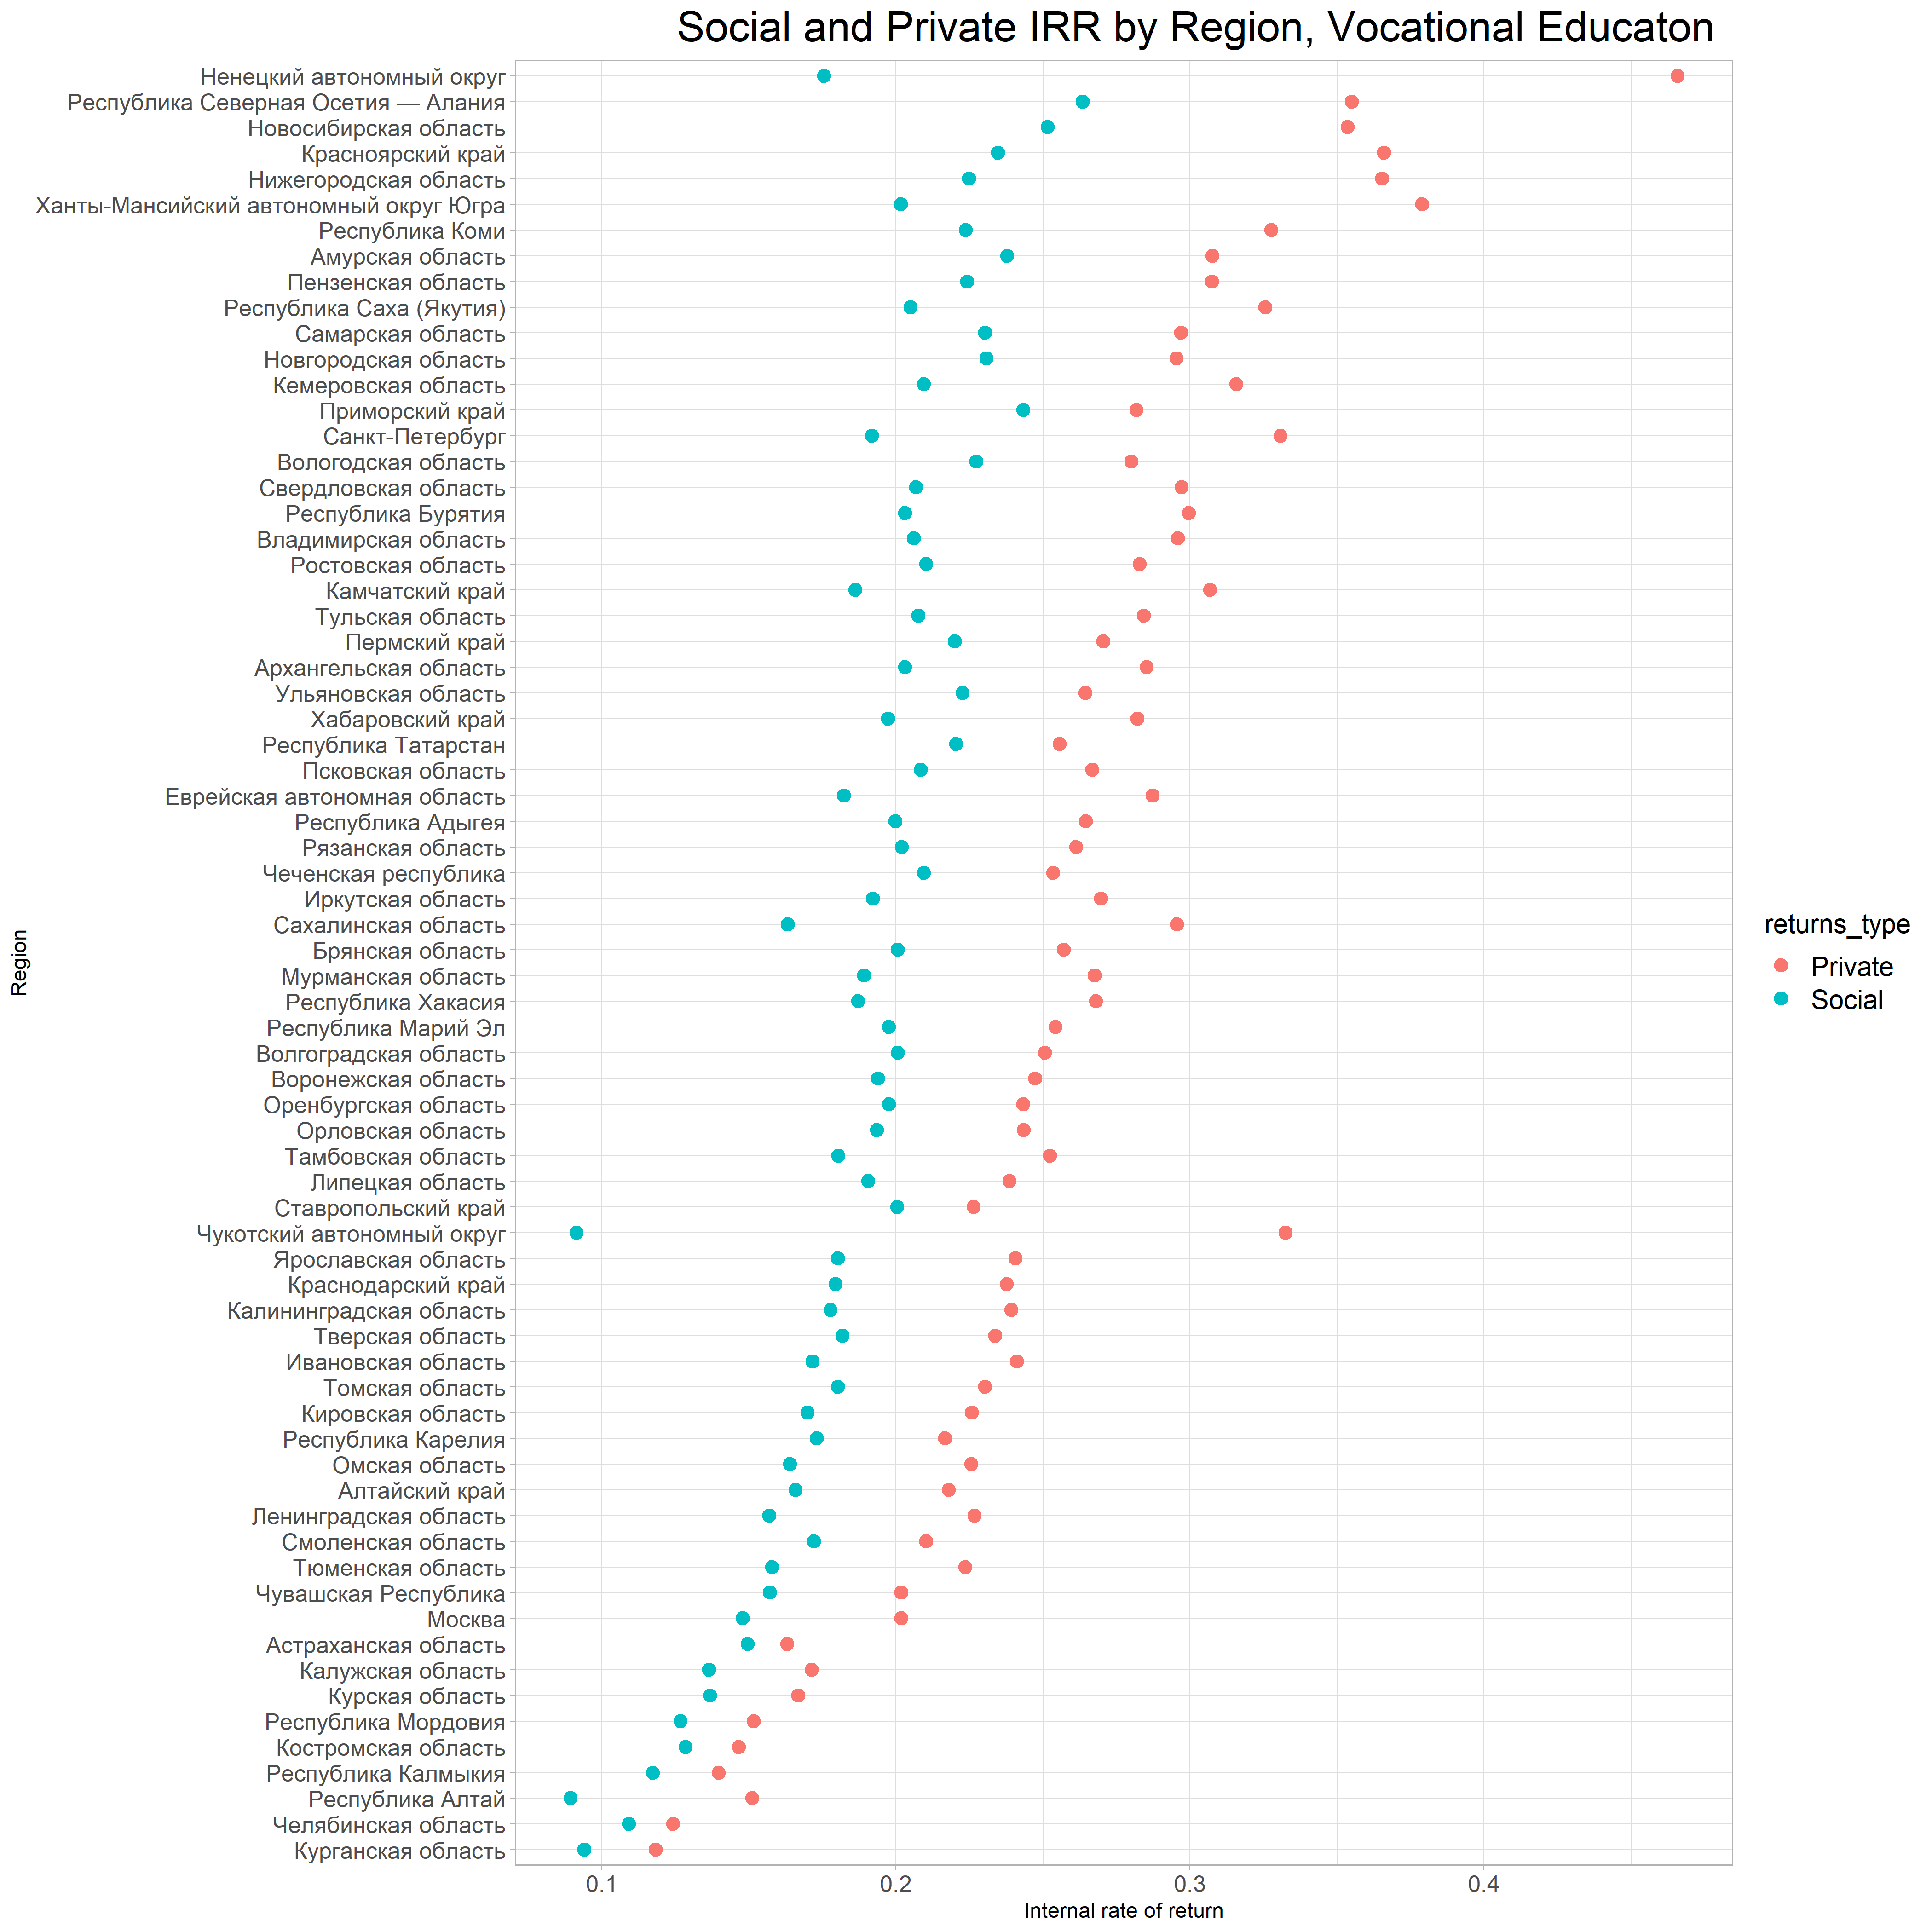
\includegraphics[scale=0.55]{returns_by_region_plot2.png}
			% plot 1
		\end{minipage}
			\caption{Social and Private Returns to Education - Vocational Education}\label{fig:1.3}
	\end{figure}

	\begin{figure}[htbp!]
\begin{minipage}[b]{1\linewidth}
			\centering
			%\hspace*{-0.7in}
			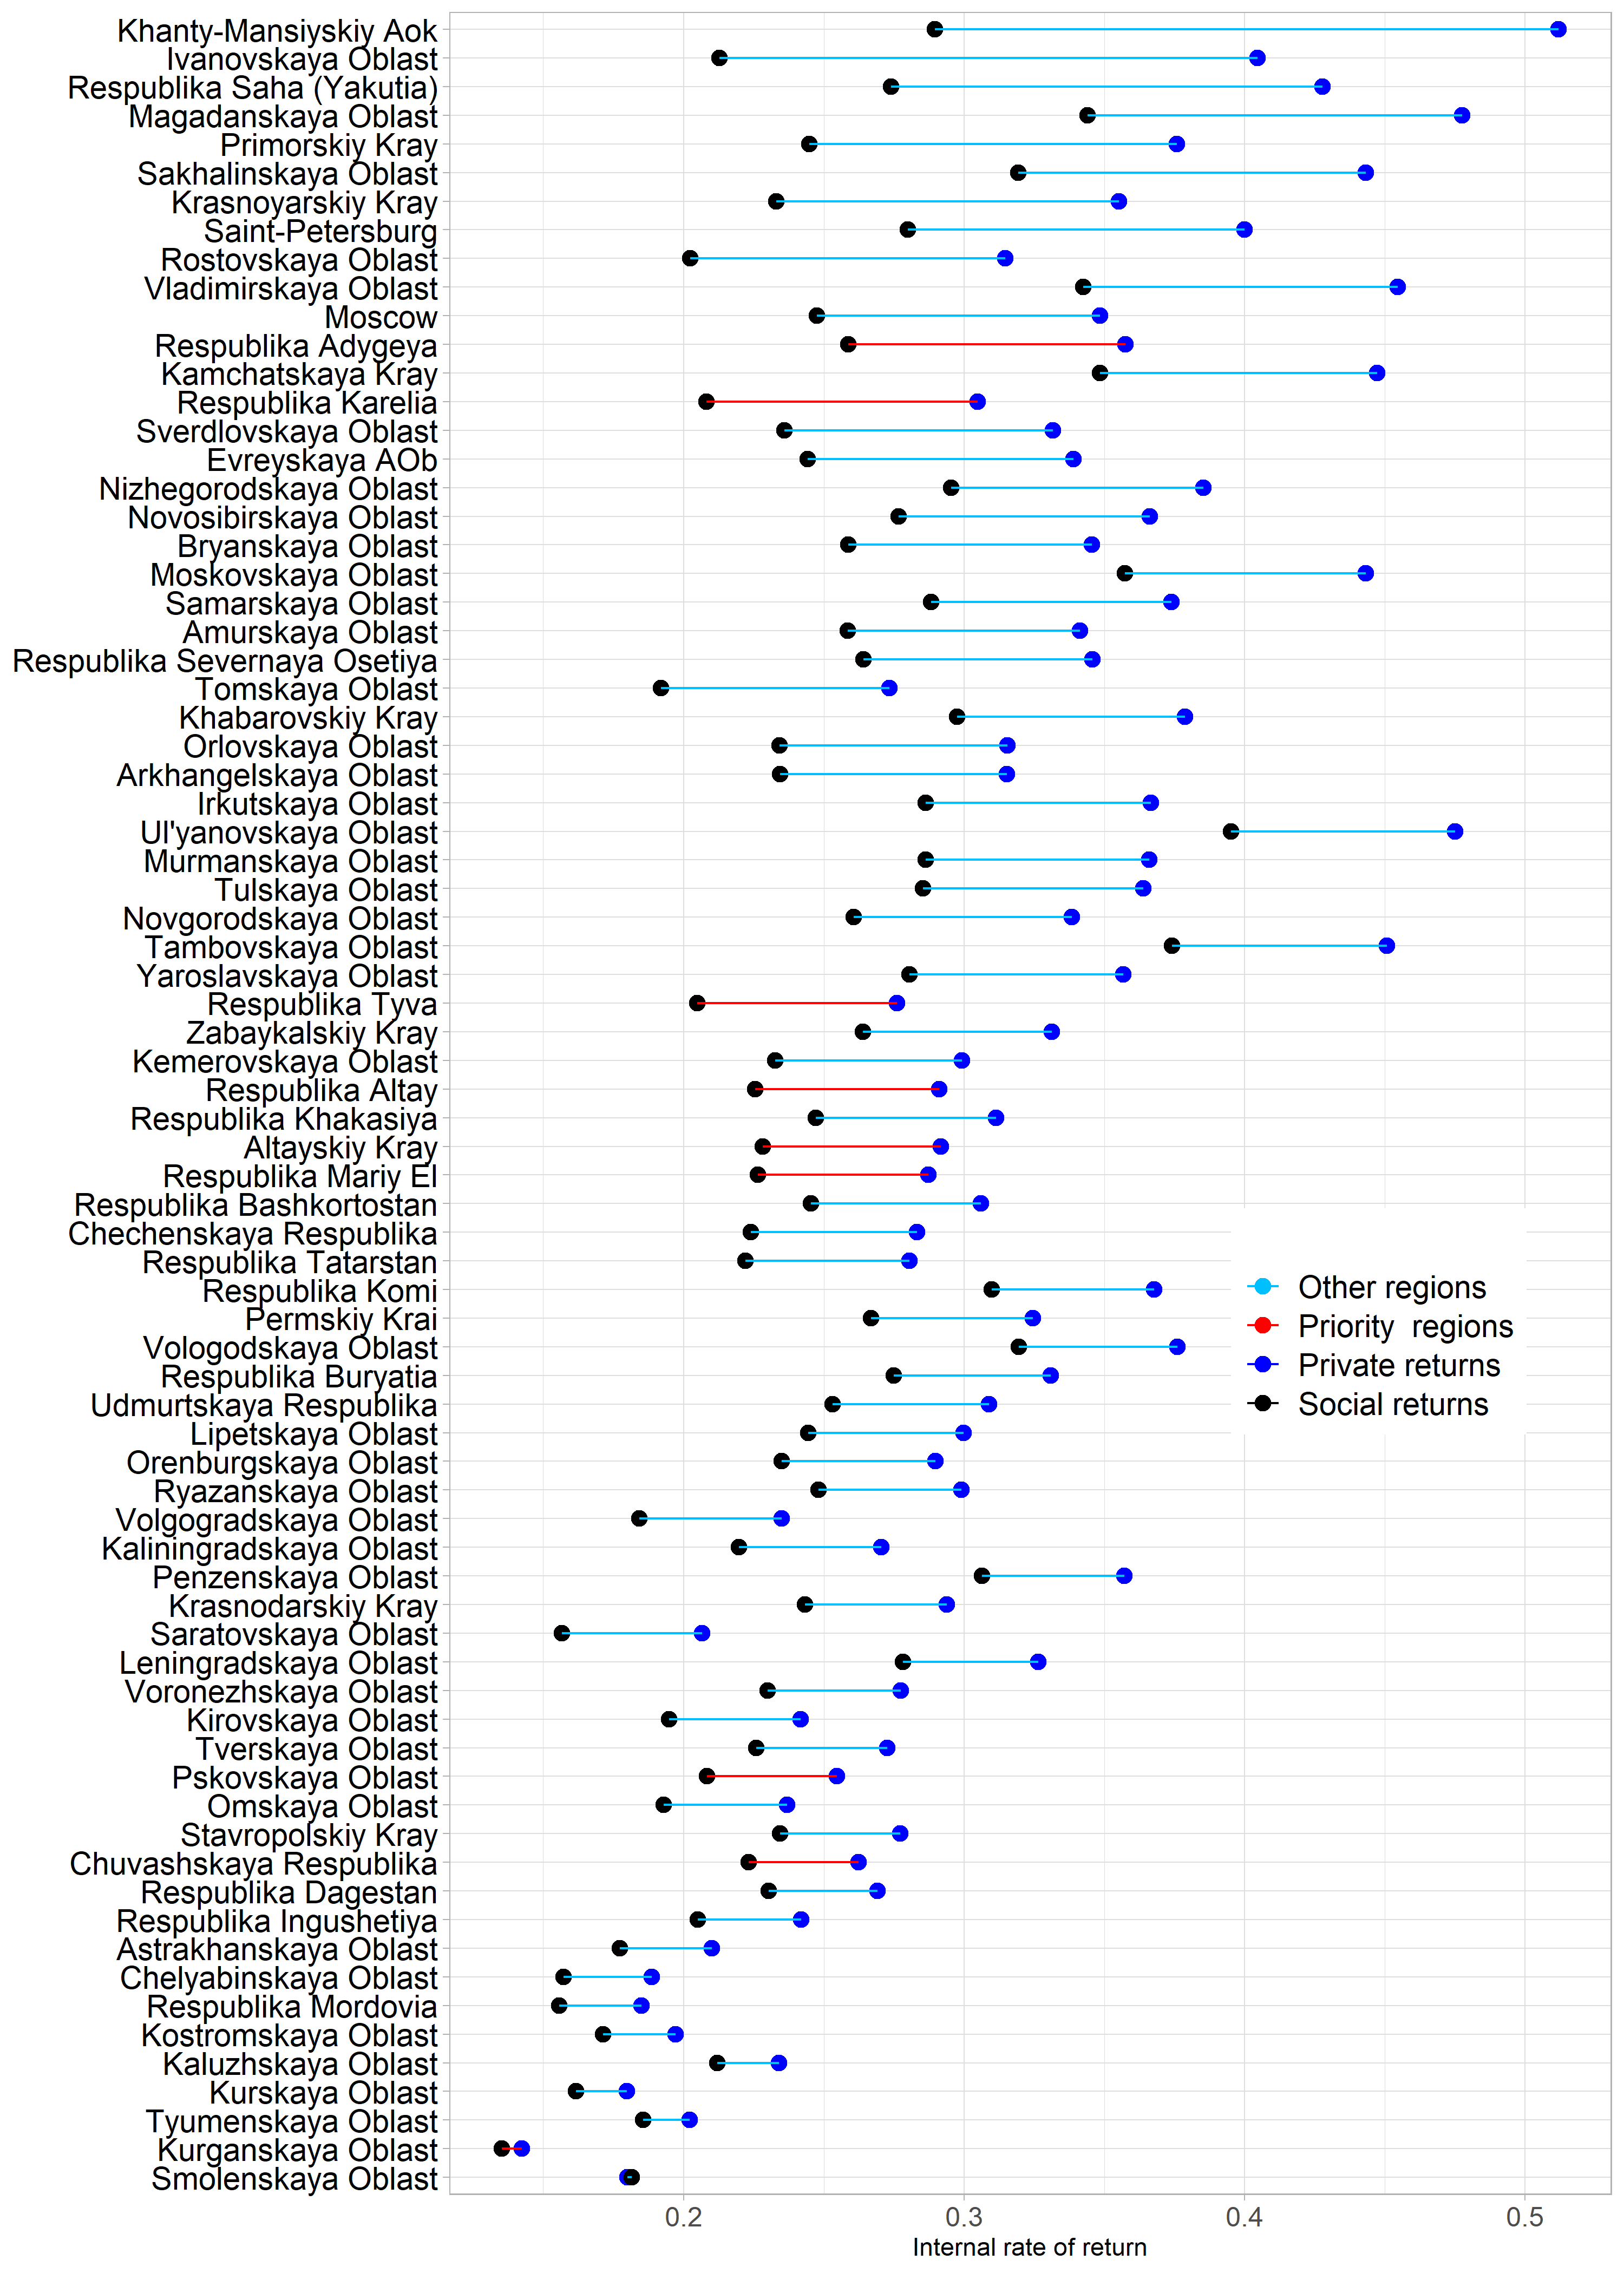
\includegraphics[scale=0.52]{returns_by_region_plot1.png}
			% plot 1
		\end{minipage}
			\caption{Social and Private Returns to Education - University Education}\label{fig:1.4}
	\end{figure}
\end{center}

\vspace{-2em}

Yet another simplification is the merging of ISCED levels 3, 4 and 5 as vocational education which entails combining different number of years after lower secondary education (Grade 9). In spite of these limitations, the returns estimates do present valid relative scenarios as the measurement problems are not specific or selective about regions and the databases are quite large, reducing sampling errors. Figure \ref{fig:1.3}  shows the returns to Vocational Education and Figure \ref{fig:1.4} the returns to Higher Education. 

\vspace{-2em}

\subsection{Estimation Results} 

Figures \ref{fig:1.3} and \ref{fig:1.4} show the gap between social and private returns to education ranges from a very small gap of 3 or 4 \% at the bottom of the graphs to 20 to 30\% gap towards the top of the graph. Since the social and private returns differ only on the cost side, the size of the gap is an indication of the extent of subsidization by the government. Subsidization of vocational education could be related to efforts of regional governments to make vocational education more attractive. The graphs also highlight the high priority regions that are slated to receive targeted support from the federal government. Working Paper No. 3 in this series provides more details about the priority regions. None of the priority regions appear amongst the top one-third of high subsidy regions for vocational education, but two of them do appear in Figure \ref{fig:1.4} for university education. It is useful to examine the subsidization of vocational and university education a bit more closely, which is done in Figure \ref{fig:1.5}. The Mincerian returns of Working Paper No. 3 are not comparable with the estimates computed here - the costs used here are averages from the years 2013 to 2017. In the Mincerian method, the only costs incorporated are the foregone earnings; the household sampled individuals would have faced a different set of costs in the past. However, Appendix \ref{tab:4.1} provides the estimates together as the valid comparison within the method is between college and university education - with the full method, the difference narrows down considerably. 

\begin{figure}[htbp!]
	\begin{minipage}[b]{.5\linewidth}
		\centering
		#\hspace*{-0.2in}
		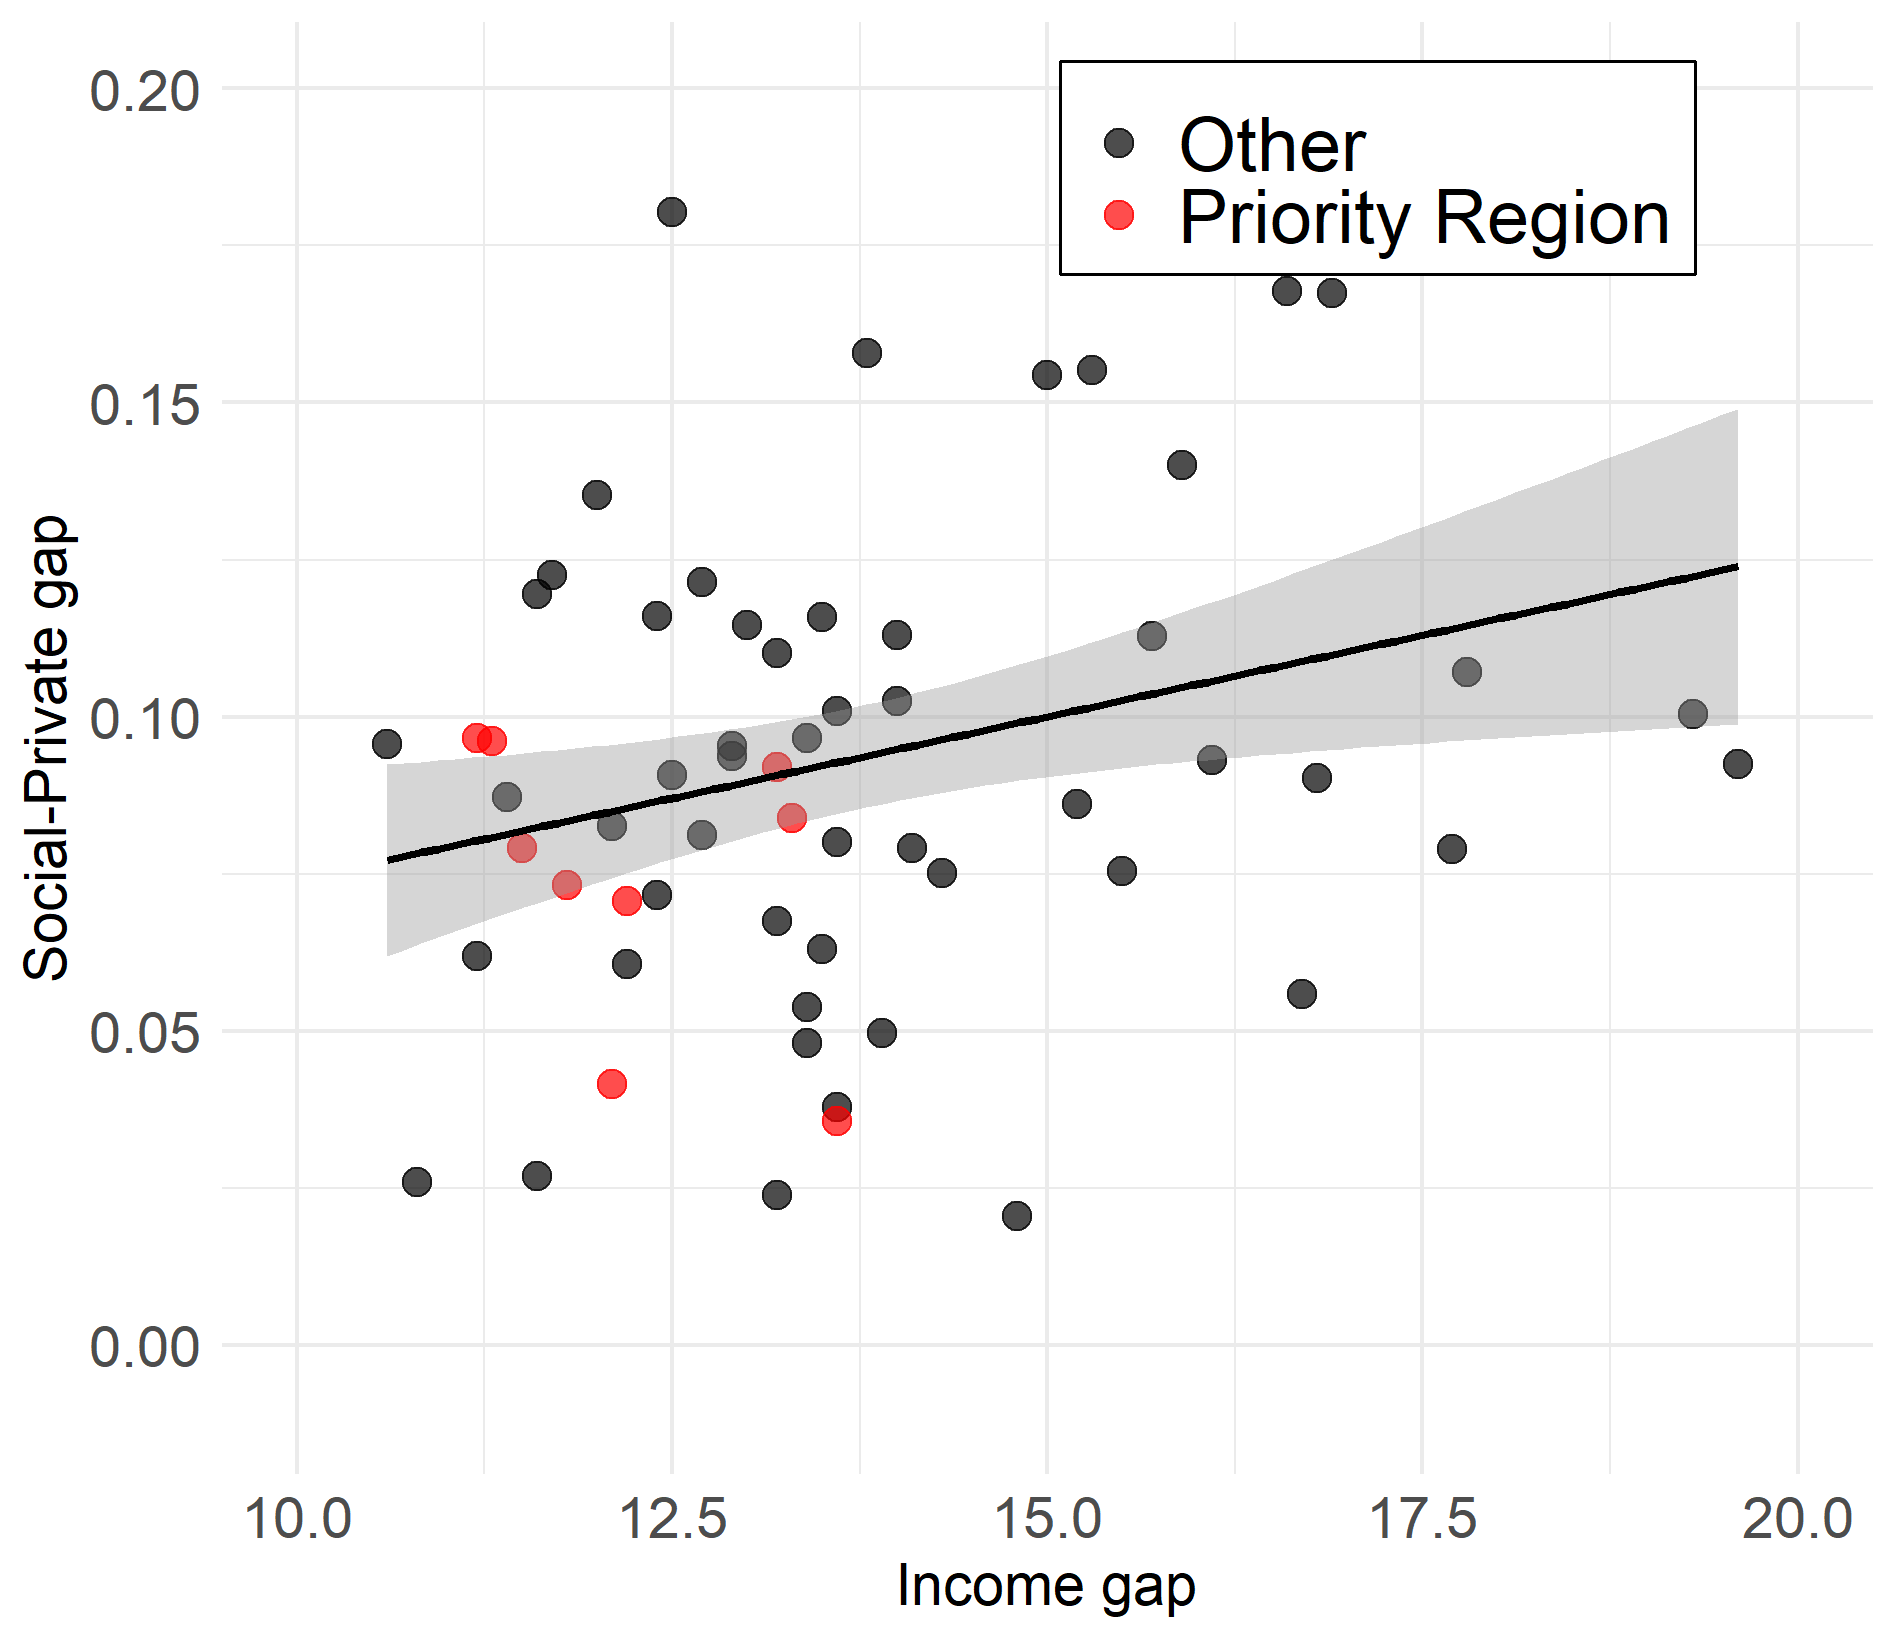
\includegraphics[width=175pt]{igap_c.png}
		% plot 1
		\subcaption{\large{College}}
	\end{minipage}
	\hfill
	\begin{minipage}[b]{.5\linewidth}
		\centering
		#\hspace*{-0.2in}
		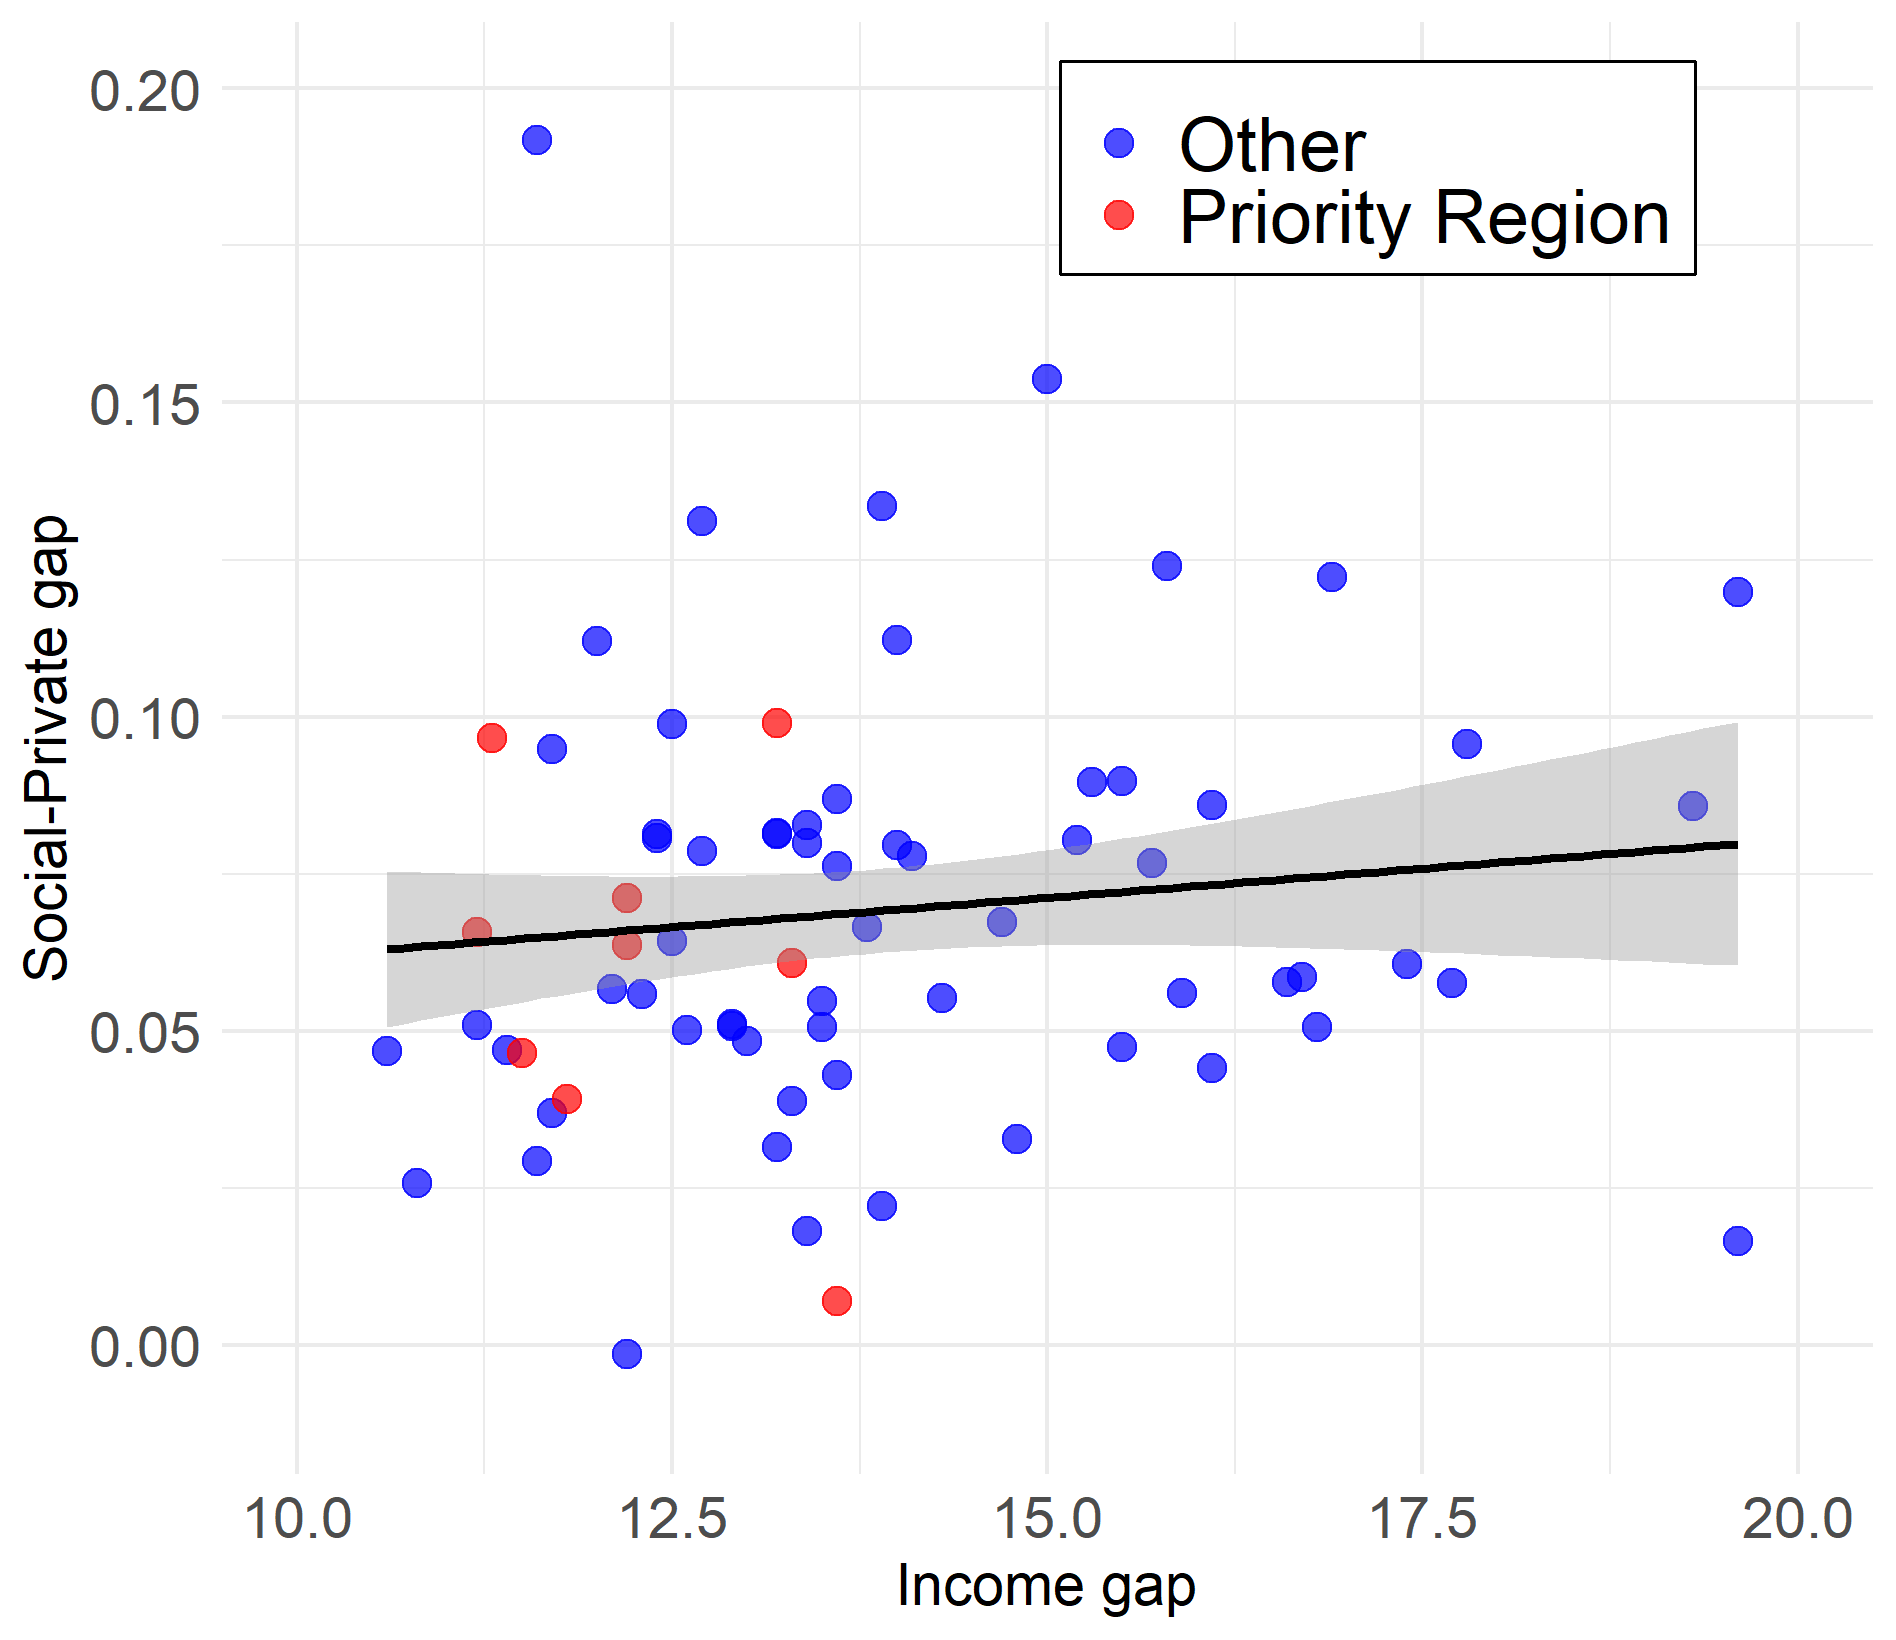
\includegraphics[width=175pt]{igap_u.png}
		% plot 2
		\subcaption{\large{University}}
	\end{minipage}
	\caption{Social-Private Returns Gap and Regional Individual Income Gap}\label{fig:1.5}
\end{figure}

The magnitude of the gap between social and private returns is lower for the university level (with mean gap of about 7\%) compared to the vocational education or college level (with mean gap of about 11\%). From a policy viewpoint, this is a correct tendency for at least two reasons - the government does want to encourage greater participation in vocational education and subsidies attract more people by lowering the price; it is also well known that there are more individuals from lower income backgrounds who attend vocational education and subsidizing such a good is progressive fiscally \footnote{An example of literature examining the choice of vocational education is  the recent World Bank report: Education Equity in Russian Federation. The report found that lower income of families of students in Grade 9 more strongly predicts vocational education choice than it does academic performance.} As discussed at length in Working Paper 3 of this series, the federal government is interested in promoting the development of the least developed regions in the country. Human capital is a crucial piece of the puzzle and spending public resources wisely would be better for growth as well as equity.  

The  International Center for the Study of Institutions and Development (ICSID) database provided by the Higher School of Economics includes data on income distribution within Russian regions \url{https://iims.hse.ru/en/csid/databases/}. We use a variable termed \textit{reg\_minckfd} that measures the ratio of mean income of the top decile of earners to the mean income of the bottom decile of earners. For this variable, Moscow region is an outlier with a value of 26 times income of 10th decile as compared to the first decile and the graph shows regions only for the rest of the range, from 10 times to 20 times on the x-axis. The gap between social and private returns is presented on the y-axis, the point representing each region is only a central tendency. Figure\ref{fig:1.5} indicates a slightly more positive slope for vocational education (in the left panel) as compared to university education. It can also be seen that the red points representing priority regions in both of the panels lie mostly below the black least squares regression line which is shown with a shaded 90\% confidence interval.

\vspace{-2em}

\section{Returns at Institutional Level for Vocational Education and Universities} 

\subsection{Descriptives}

We turn now to the data from graduate.edu.ru on salaries of graduates from colleges and universities. Whether to study in a vocational college or a university, what course of specialization to choose, and which is the optimal institute for an individual are complex decisions. However, it is straightforward to conceptualize the choice as an investment decision. In the present case, even though we only have three years of data regarding graduates, we show that the information can be productively utilized. 

\begin{figure}[htbp!]
	\begin{minipage}[b]{.5\linewidth}
		\centering
		#\hspace*{-0.2in}
		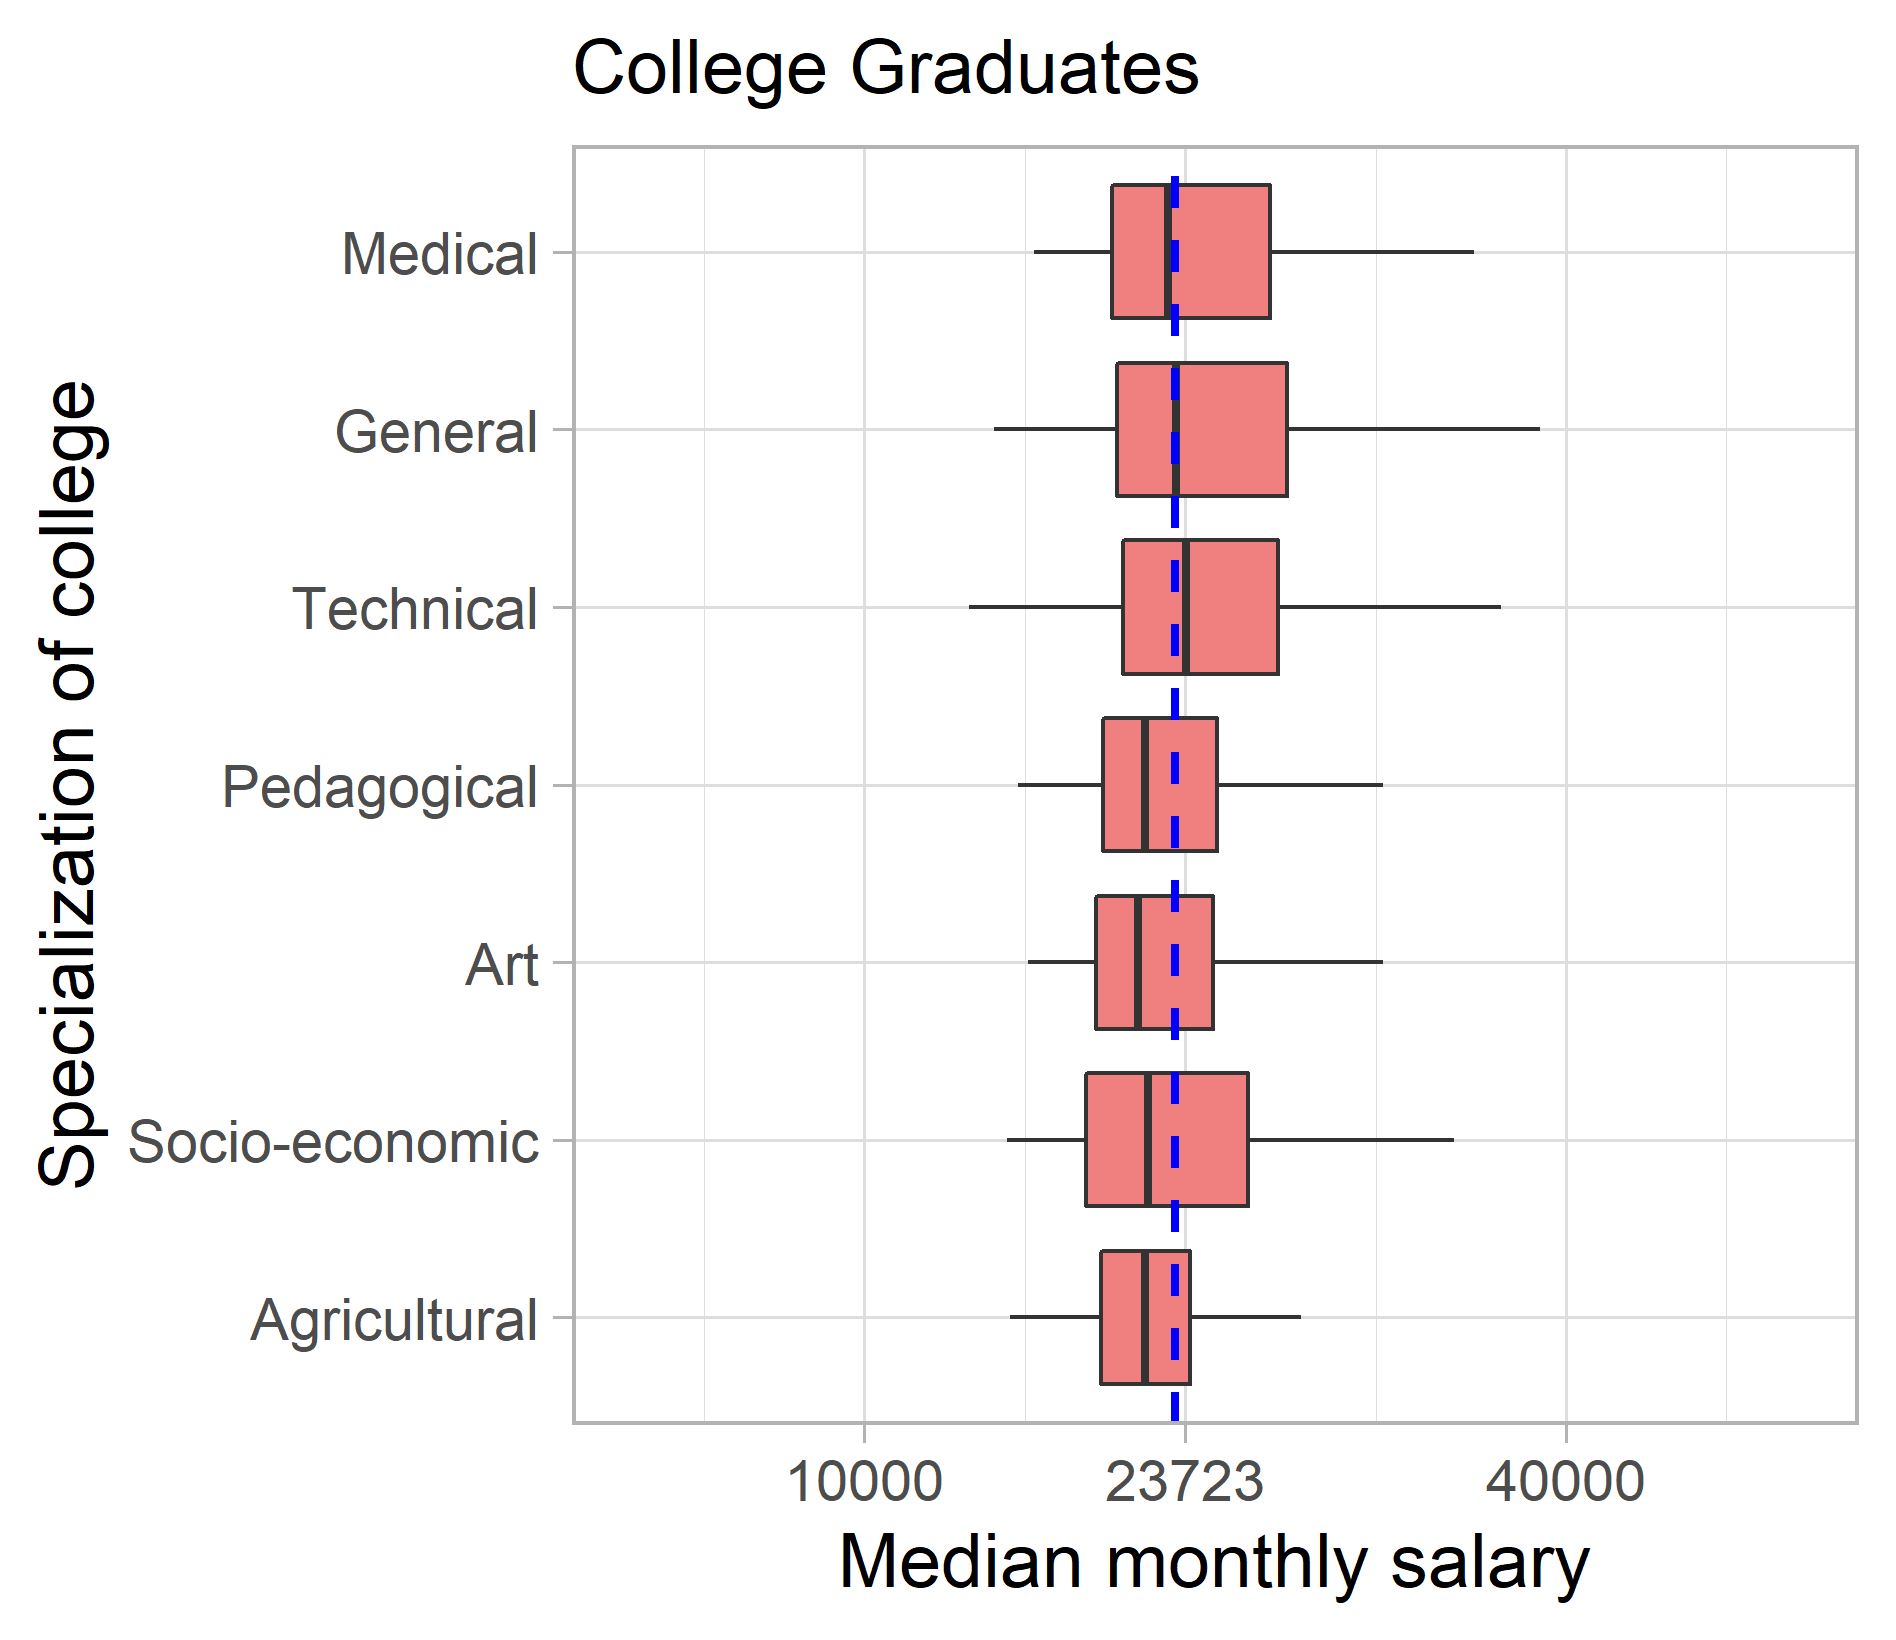
\includegraphics[width=150pt]{sal_spnc.png}
		% plot 1
		\subcaption{\large{College}}
	\end{minipage}
	\hfill
	\begin{minipage}[b]{.5\linewidth}
		\centering
		#\hspace*{-0.2in}
		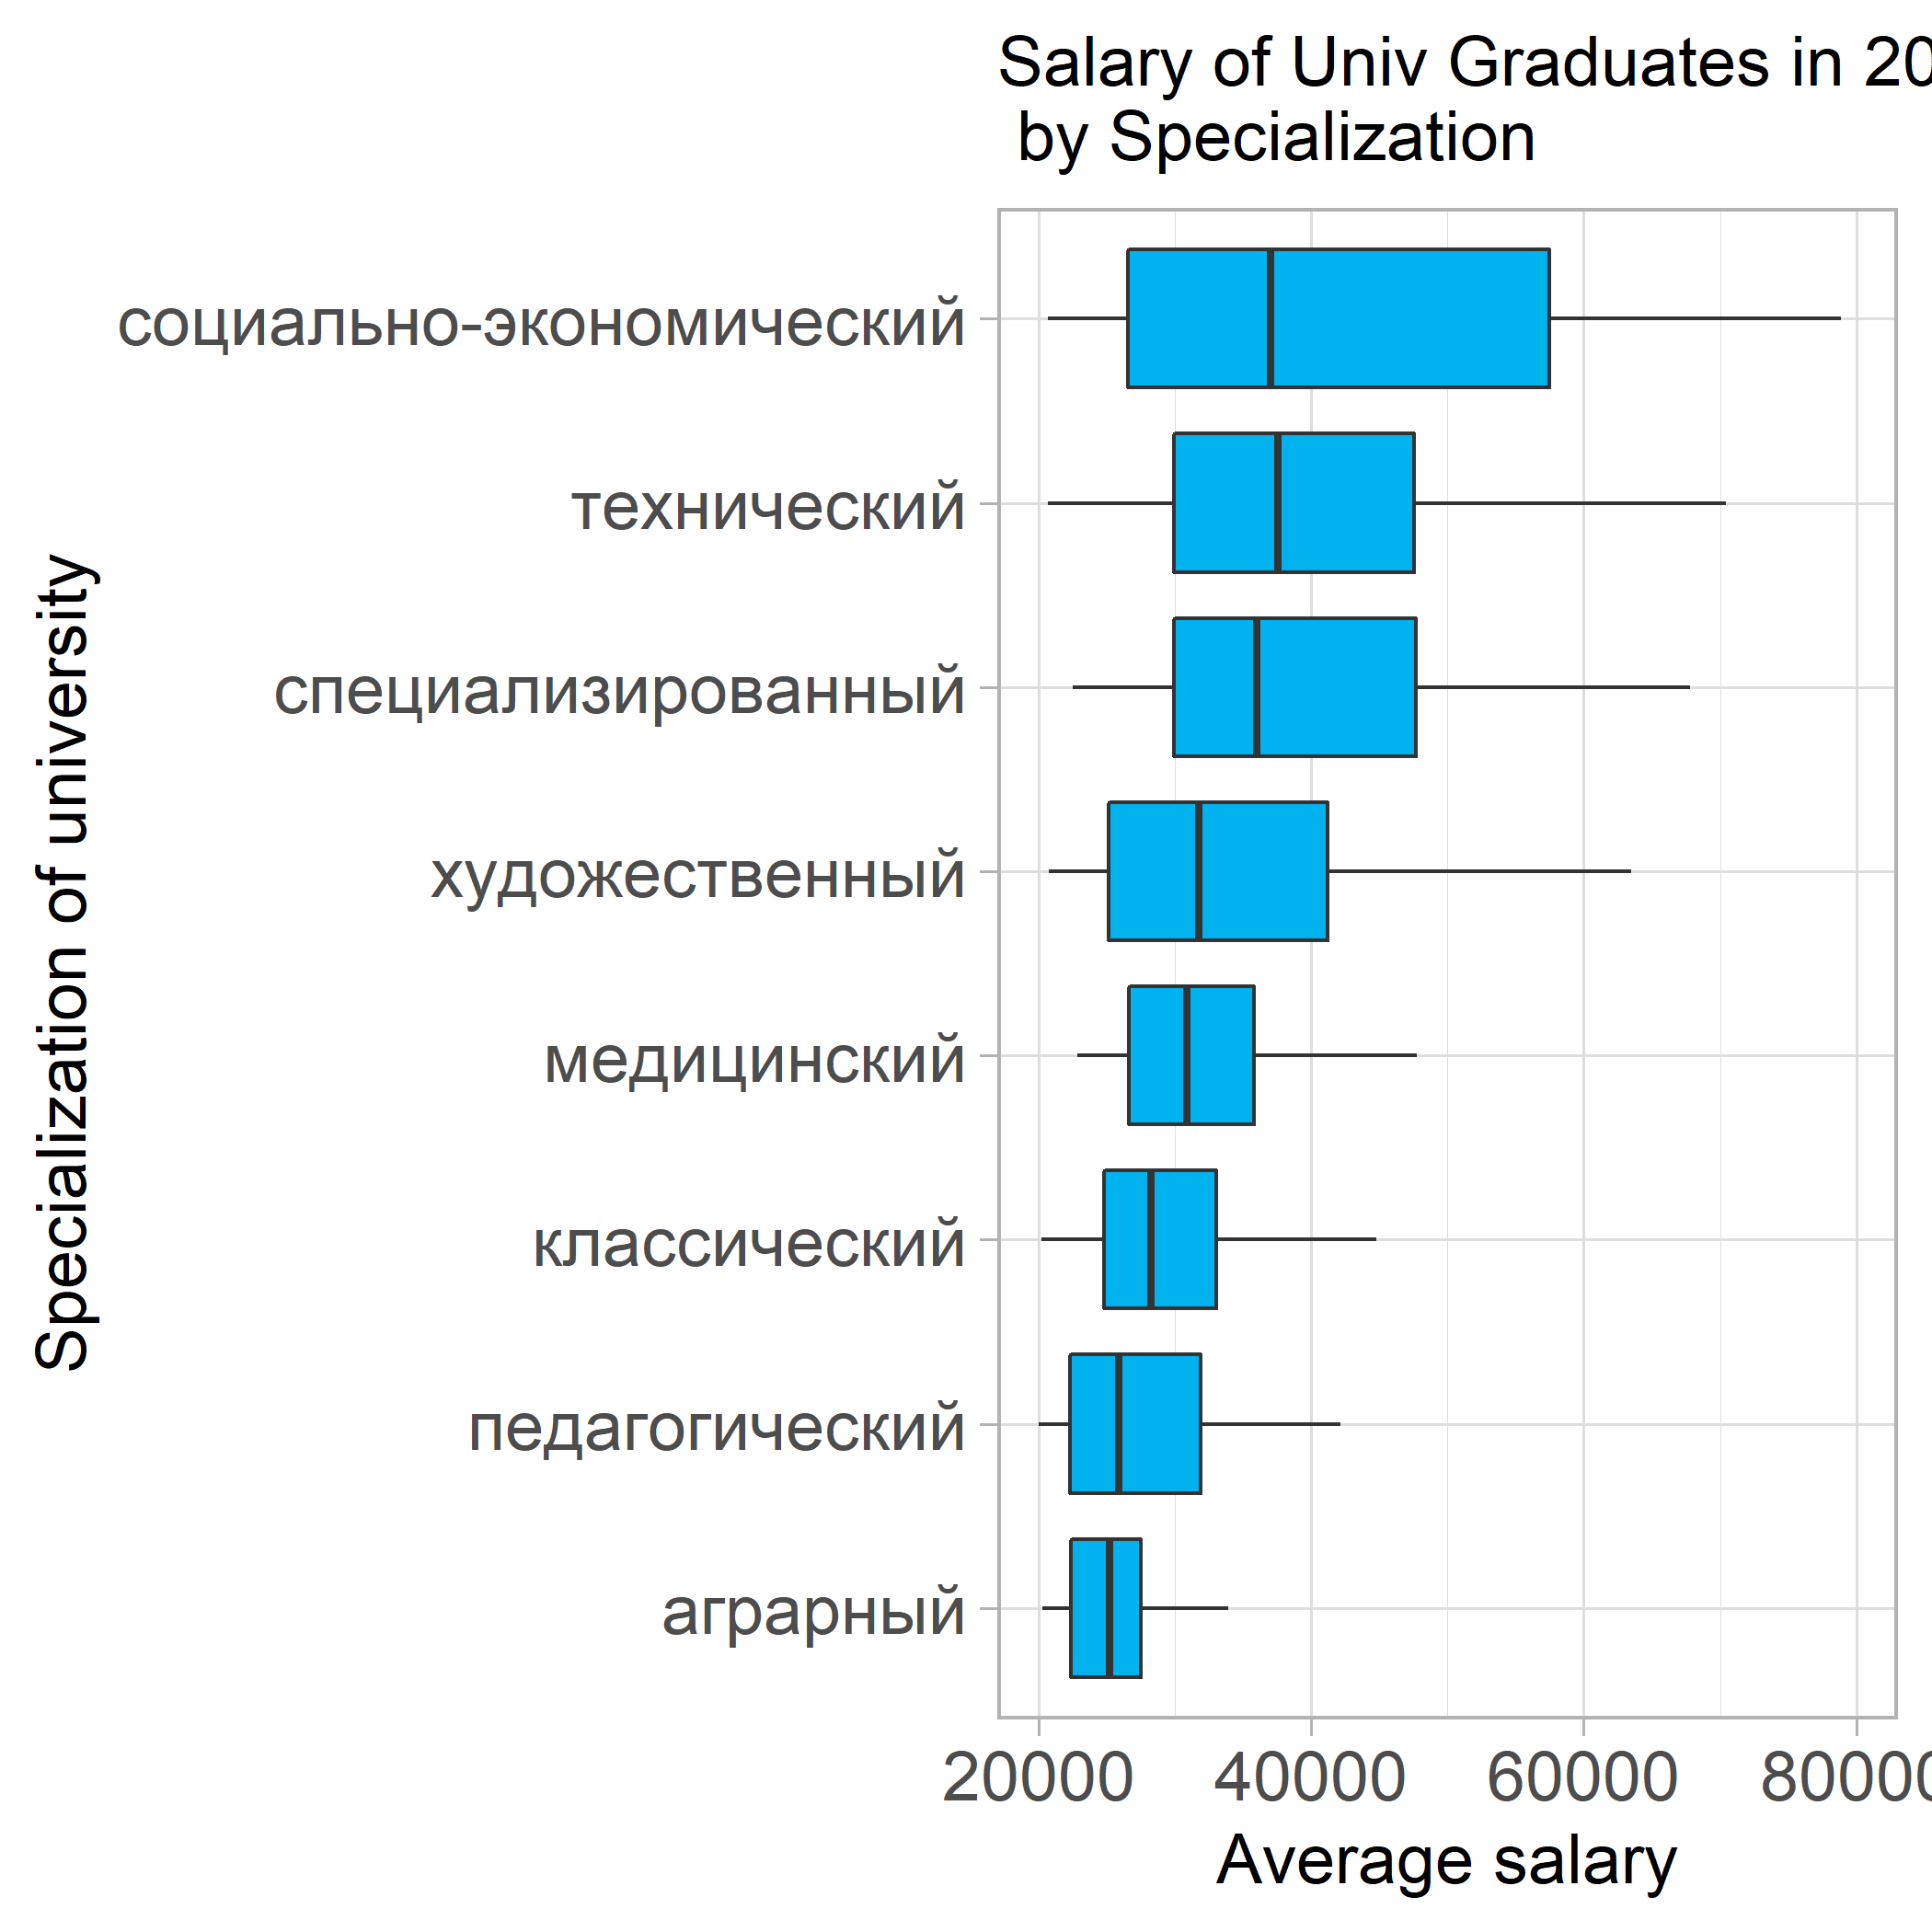
\includegraphics[width=150pt]{sal_spnu.png}
		% plot 2
		\subcaption{\large{University}}
	\end{minipage}
	\caption{Monthly Salary in year 2014 of Graduates by Study Specialization}\label{fig:1.6}
\end{figure}

Figure \ref{fig:1.6} provides a summary of the graduate salary information for 2014 (in 2016 rubles) by broad area of specialization, separately for those who attended vocational college or university. These are the categories of colleges or universities only as we do not have information by department or faculty within a college or university. Overall medians are also presented that show a median graduate monthly salary of 23,723 rubles for vocational education and 30,521. The boxplots ends are the 25th percentile and 75th percentile. It is immediately apparent from Figure \ref{fig:1.6} that the dispersion of salaries is lower for vocational education graduates, both across and within specializations. For university graduates on the other hand, even the 75th percentile wage for some specializations, such as agrarian or pedagogical, barely make it to the overall median. Data from graduate.edu is available for 2014 graduates for two more years. Interestingly, patterns of variation can be seen even in this short interval, which generates confidence in using the data to compare across institutions. Appendix Figure \ref{fig:7.6} shows a plot of real salary increases from 2014 to 2016 for university graduates who graduated in 2014. As might be expected, specialized scientific and technical disciplines garnered the biggest increases.  In some cases there were zero increases or even declines, with `education and pedagogical sciences' one of the notable cases registering a decline. Low starting salaries for pedagogical specializations may persist over an early probation period of two to three years, possibly be made up later in the career. If a longer time period of data had been available from graduate.edu, there might have been some movement in the relative placement of the specializations.  However, it seems unlikely that there would have been large scale movements. The information presented in Appendix Figure \ref{fig:7.6} makes intuitive sense and provides some reassurance that the availability of only three years or earnings data does not make it totally dominated by noise. This also makes sense given the fact that the raw data on which the information is based is almost a census data, with graduate.edu.ru publishing institutional level means based on salaries from over 1 million individual records. 

\vspace{-2em}

\subsection{Social and Private Returns by Institution}

Productive investments, such as education in a college or university, can 
be evaluated or ranked in terms of optimality by examining the cash flows 
that result from alternative investment choices. There is a negative cash 
flow during the period of study - made up of direct costs such as tuition 
fees, transportation and textbooks, as well as the indirect costs of 
foregone income. In considering social costs these include the subsidies 
provided by government so that students pay low or sometimes no tuition. In 
the Russian Federation, some students are completely subsidized while other 
students pay partial or full fees. In the computations presented in this 
paper, we only use institution level means for both private and social 
costs. Some of the data points appear to be outliers and we `trim' the 
bottom and top 1\% of observations. We also exclude colleges with less than 
50 students and universities with less than 100 students. As stated before, 
there are a number of simplifications used to compute unit costs per 
student from the aggregate financial information of a college or 
university. For foregone earnings we utilize the regional level mean 
earnings for those who did not go beyond Secondary education. 

The negative stream of cash flows at the beginning are evaluated against the positive stream of cash flows when graduates begin to earn in the labor market. Employment is a probabilistic outcome but we do not have information about the specific employment rate for each institute. The classical internal rate of return would be the discount rate applied to the future stream of lifetime earnings to equal the value of the negative stream during the schooling period. The same method can be applied to calculate an internal rate of return with only three years of positive earnings. Even though most rates are negative, the method still yields a relative ranking of colleges and separately, of universities. The main purpose of this analysis is to provide the processed information to the public. The graduate.edu.ru website provides useful information in varied forms about the salaries of graduates. This information would become even more valuable when combined with the cost information to provide an internal rate of return. If updates can be made to the graduate.edu with more recent salary data since 2016, the internal rate of return can be updated. For dedicated evidence based decision making, it is also possible in the future to get more accurate information ion the cost side. For instance, it would be very useful to build on the bus.gov.ru data used here with a primary data collection effort. 

At the present time, we are providing the list of colleges and universities with the private and social rates of return and the underlying data about cost and graduate salaries. Table \ref{tab:1.3} provides a summary list of top and bottom ten. Figure \ref{fig:1.17} provides depiction on a map as a demonstration of a possible user interface of the data, since the data incorporates GPS coordinates. Figure \ref{fig:1.18}  indicates social rates of return by type of college and university. Pedagogical and agricultural universities do better on this measure as compared to their performance on salary levels. 




\begin{table}
\def\arraystretch{0.8} 
%\setlength\arrayrulewidth{1pt}
    \centering
		\caption{Social and Private Returns by Instititution: Top and Bottom 10}
		\label{tab:1.3}\\
    \begin{tabular}{|p{.75cm}|p{.75cm}|p{7cm}|p{3cm}|R{1.25cm}|}
    \hline
\multicolumn{5}{|c|}{\textbf{Top 10 Colleges}} \\ \hline
social  & private  & Name & Region  & Number graduates\\ \hline
0.13 & 0.35 & Samara Power Engineering College & Samarskaya Oblast & 140 \\ 
0.13 & 0.22 & Tomsk Polytechnic Technical School & Tomskaya Oblast & 306 \\ 
0.12 & 0.24 & Novocherkassk Geological Exploration College & Rostovskaya Oblast & 244 \\ 
0.12 & 0.28 & Vilyui Technical School & Resp. Sakha (Yakutia) & 156 \\ 
0.11 & 0.21 & Kiselevsky Mining College & Kemerovskaya Oblast & 280 \\ 
0.11 & 0.25 & Higher Banking School & Saint-Petersburg & 229 \\ 
0.11 & 0.24 & Industrial and Technological College & Saint-Petersburg & 305 \\ 
0.10 & 0.18 & Perm Oil College & Permskiy Krai & 171 \\ 
0.10 & 0.30 & Yakut Road Technical School & Resp. Sakha (Yakutia) & 220 \\ 
0.10 & 0.19 & Sakhalin Indus. \& Economic College & Sakhalinskaya Oblast & 489 \\ 
-0.01 & 0.01 & Tomsk Industrial University & Tomsk & 6655 \\ \hline 
\multicolumn{5}{|c|}{\textbf{Bottom 10 Colleges}} \\ \hline
social  & private  & Name & Region  & Number graduates \\ \hline
-0.32 & -0.04 & Abakan Construction College & Respublika Khakasiya & 70 \\ 
-0.32 & -0.24 & Ichalkovsky Pedagogical College & Respublika Mordovia & 62 \\ 
-0.32 & -0.19 & Ozersk Technical College & Chelyabinskaya Oblast & 154 \\ 
-0.32 & 0.04 & Metrostroy College & Saint-Petersburg & 55 \\ 
-0.32 & -0.16 & Kaluga Technical College & Kaluzhskaya Oblast & 154 \\ 
-0.33 & -0.02 & Yemelyanov Road Construction Technical School & 
Krasnoyarskiy Kray & 73 \\ 
-0.33 & -0.14 & Technology College No. 21 & Moscow & 216 \\ 
-0.33 & 0.12 & Sakhalin Technical School of Agricultural Mechanization & Sakhalinskaya Oblast & 82 \\ 
-0.34 & 0.15 & Krasnoselsky College & Saint-Petersburg & 74 \\ 
-0.34 & -0.02 & Krasnodar Pedagogical College & Krasnodarskiy Kray & 148 \\ \hline
\multicolumn{5}{|c|}{\textbf{Top 10 Universities}} \\ \hline
social  & private  & Name & Region  & Number graduates \\ \hline
0.07 & 0.09 & Buryat State Agricultural Academy & Respublika Buryatia & 415 \\ 
0.05 & 0.09 & Russian State Univ. of Tourism and Service & Moskovskaya Oblast & 3019 \\ 
0.05 & 0.07 & Tyumen Industrial University & Tyumenskaya Oblast & 6655 \\ 
0.04 & 0.07 & Samara Sate Univ. of Economics & Samarskaya Oblast & 1826 \\ 
0.04 & 0.20 & North-Eastern State University & Magadanskaya Oblast & 573 \\ 
0.04 & 0.10 & Siberian State Industrial University & Kemerovskaya Oblast & 1727 \\ 
0.04 & 0.13 & Samara State Technical University & Samarskaya Oblast & 2879 \\ 
0.03 & 0.09 & Siberian State Univ. of Geosystems \& Technologies & Novosibirskaya Oblast & 1768 \\ 
0.03 & 0.10 & Kamchatka State Technical University & Kamchatskaya Kray & 826 \\ 
0.02 & 0.15 & Arctic State Inst. of Culture and Arts & Resp. Sakha (Yakutia) & 366 \\ 
\hline
\multicolumn{5}{|c|}{\textbf{Bottom 10 Universities}} \\ \hline
social  & private  & Name & Region  & Number graduates \\ \hline
-0.29 & -0.18 & Samara State Medical University  & Samarskaya Oblast & 1169 \\ 
-0.30 & -0.13 & Pirogov Russian National Research Medical University & Moscow & 1165 \\ 
-0.30 & -0.22 & Astrakhan State Univ. of Arch. \& Civil Eng. & Astrakhanskaya Oblast & 282 \\ 
-0.30 & -0.10 & Stroganov Moscow State Acad. of Art \& Industry & Moscow & 196 \\ 
-0.30 & -0.17 & Siberian State Medical University  & Tomskaya Oblast & 630 \\ 
-0.31 & -0.16 & Bryansk State Agrarian University & Bryanskaya Oblast & 408 \\ 
-0.31 & -0.14 & National Research Technological University  & Moscow & 1394 \\ 
-0.32 & -0.18 & North-Western State Medical University  & Saint-Petersburg & 949 \\ 
-0.34 & -0.16 & Saratov State Conservatory & Saratovskaya Oblast & 116 \\ 
-0.35 & -0.15 & Ural State Agrarian University & Sverdlovskaya Oblast & 260 \\ 
\hline
\end{tabular}
\end{table}







\begin{figure}[htp]
	\begin{minipage}[b]{.5\linewidth}
		\centering
		\hspace*{-0.4in}
		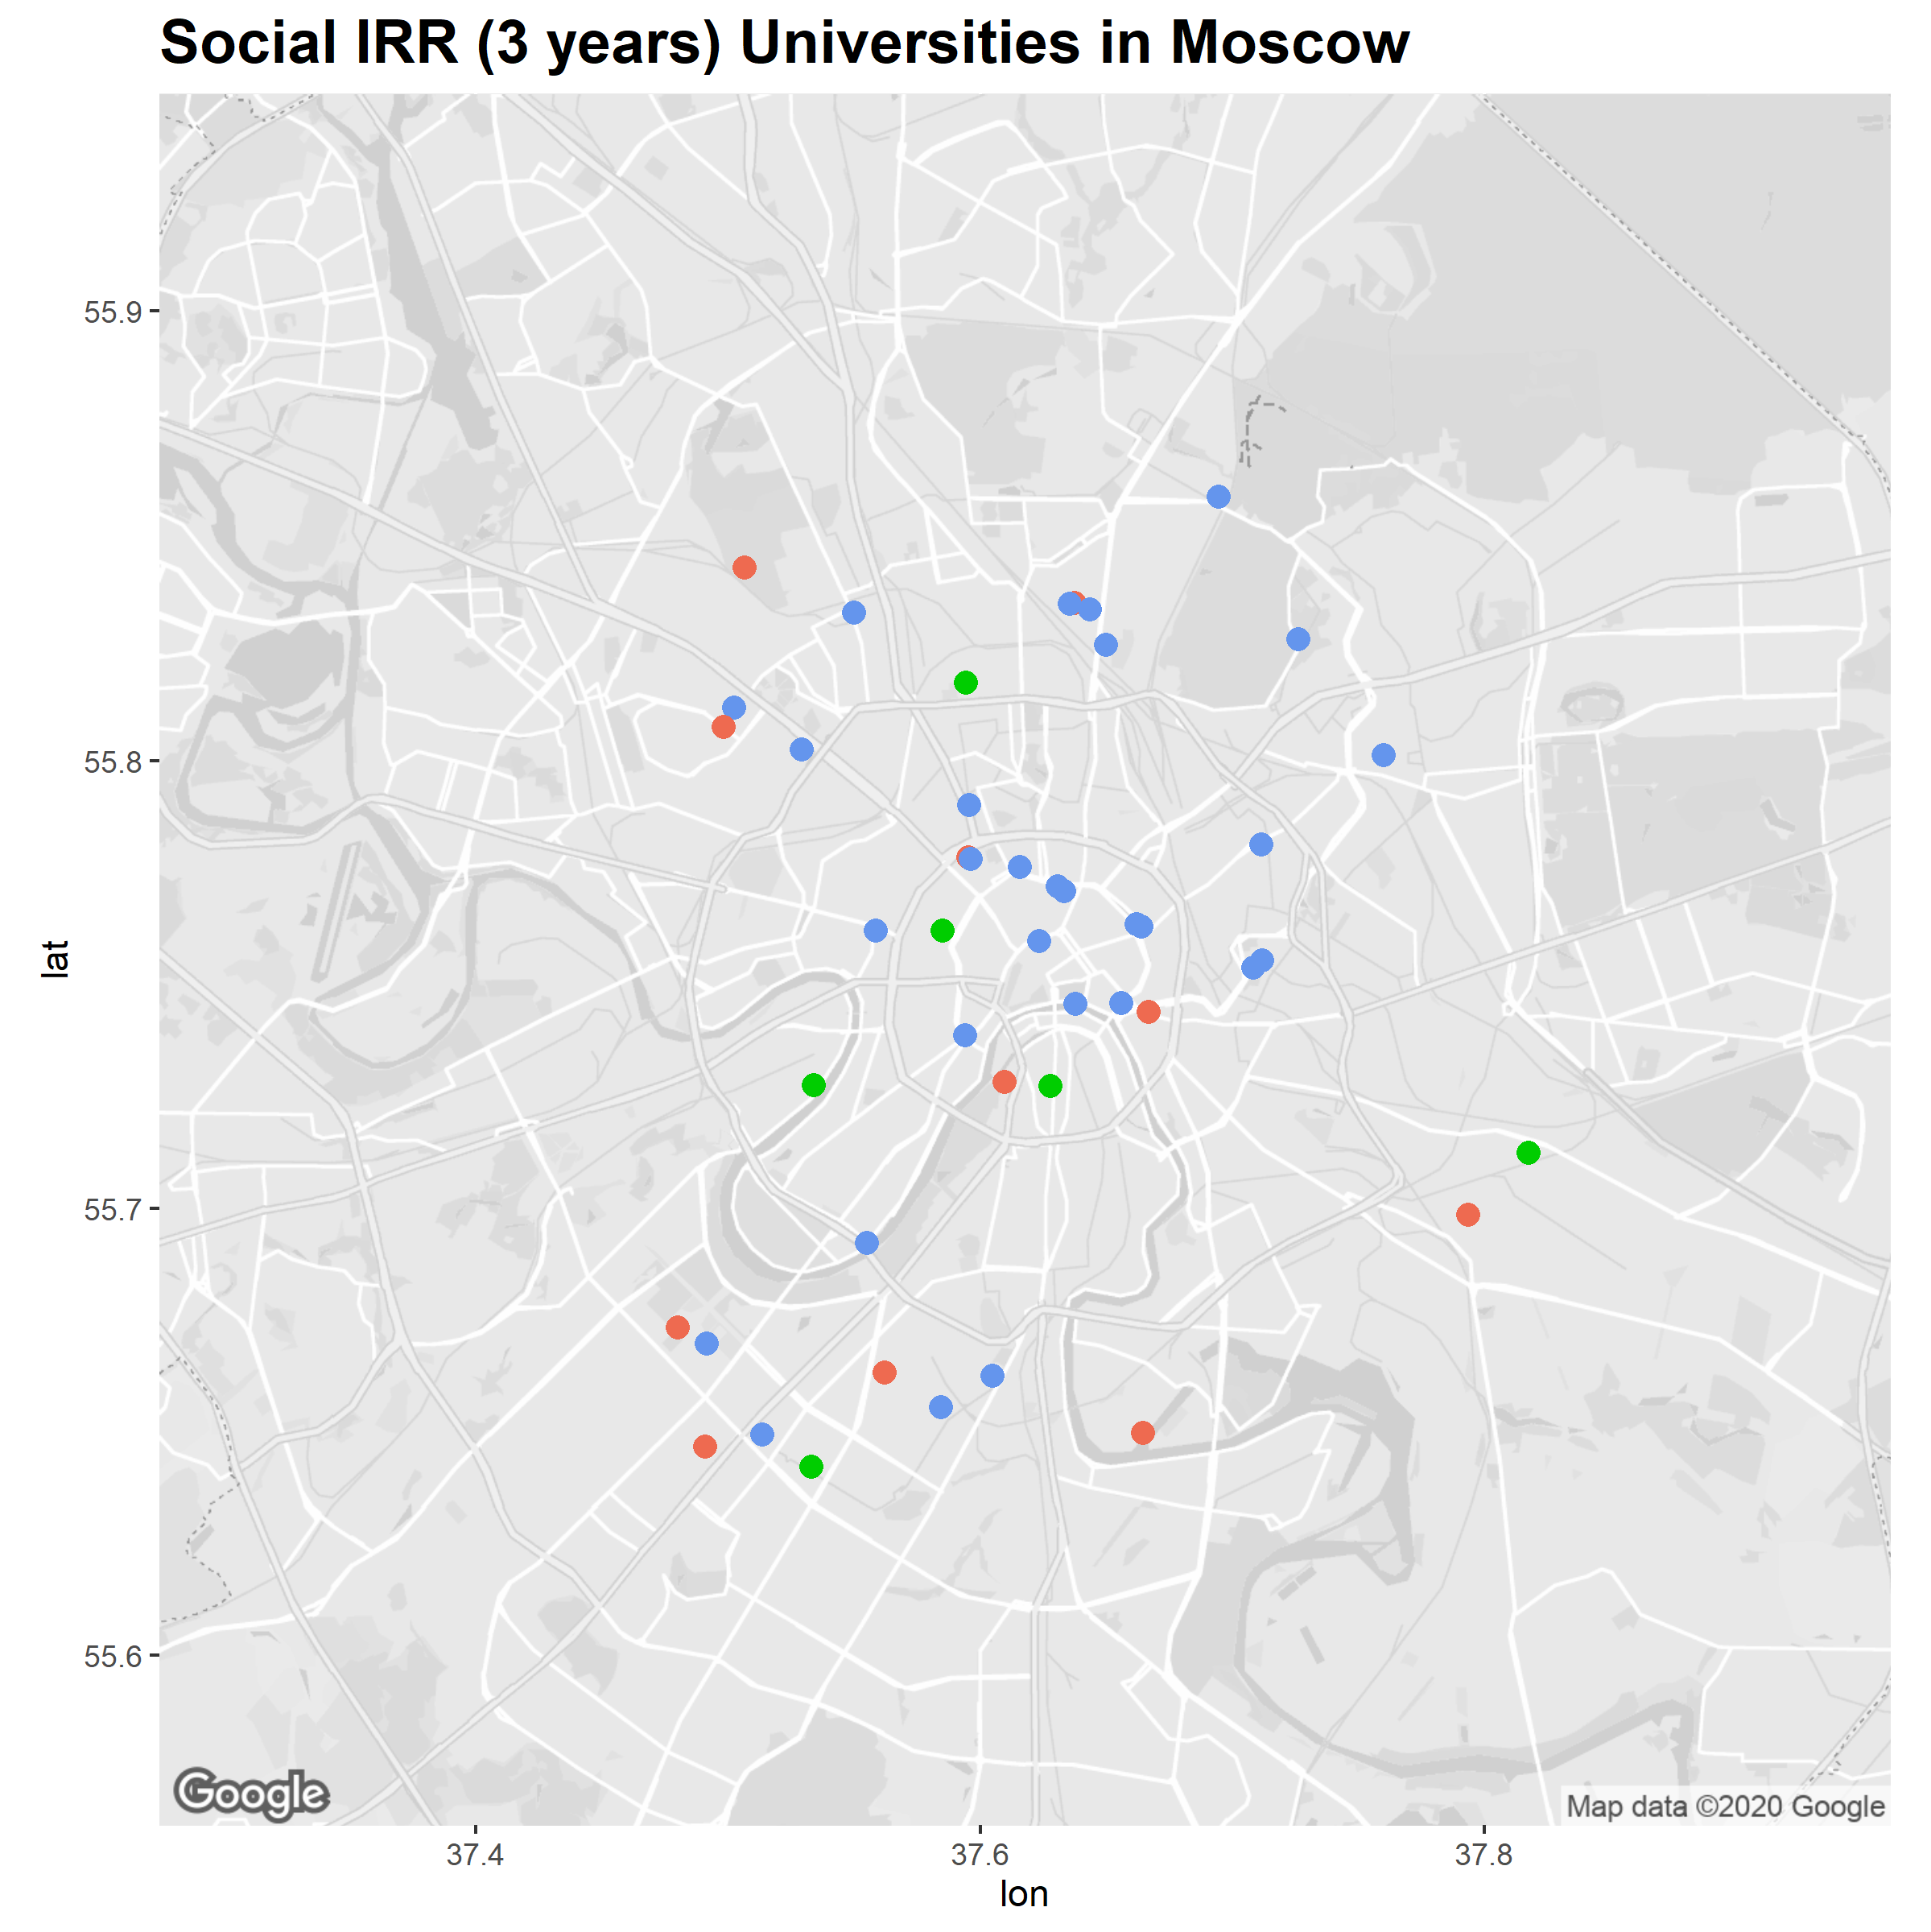
\includegraphics[width=200pt]{social_returns_moscow.png}
		% plot 1
	%	\subcaption{Moscow}\label{}
	\end{minipage}
	\hfill
	\begin{minipage}[b]{.5\linewidth}
		\centering
		\hspace*{-0.2in}
		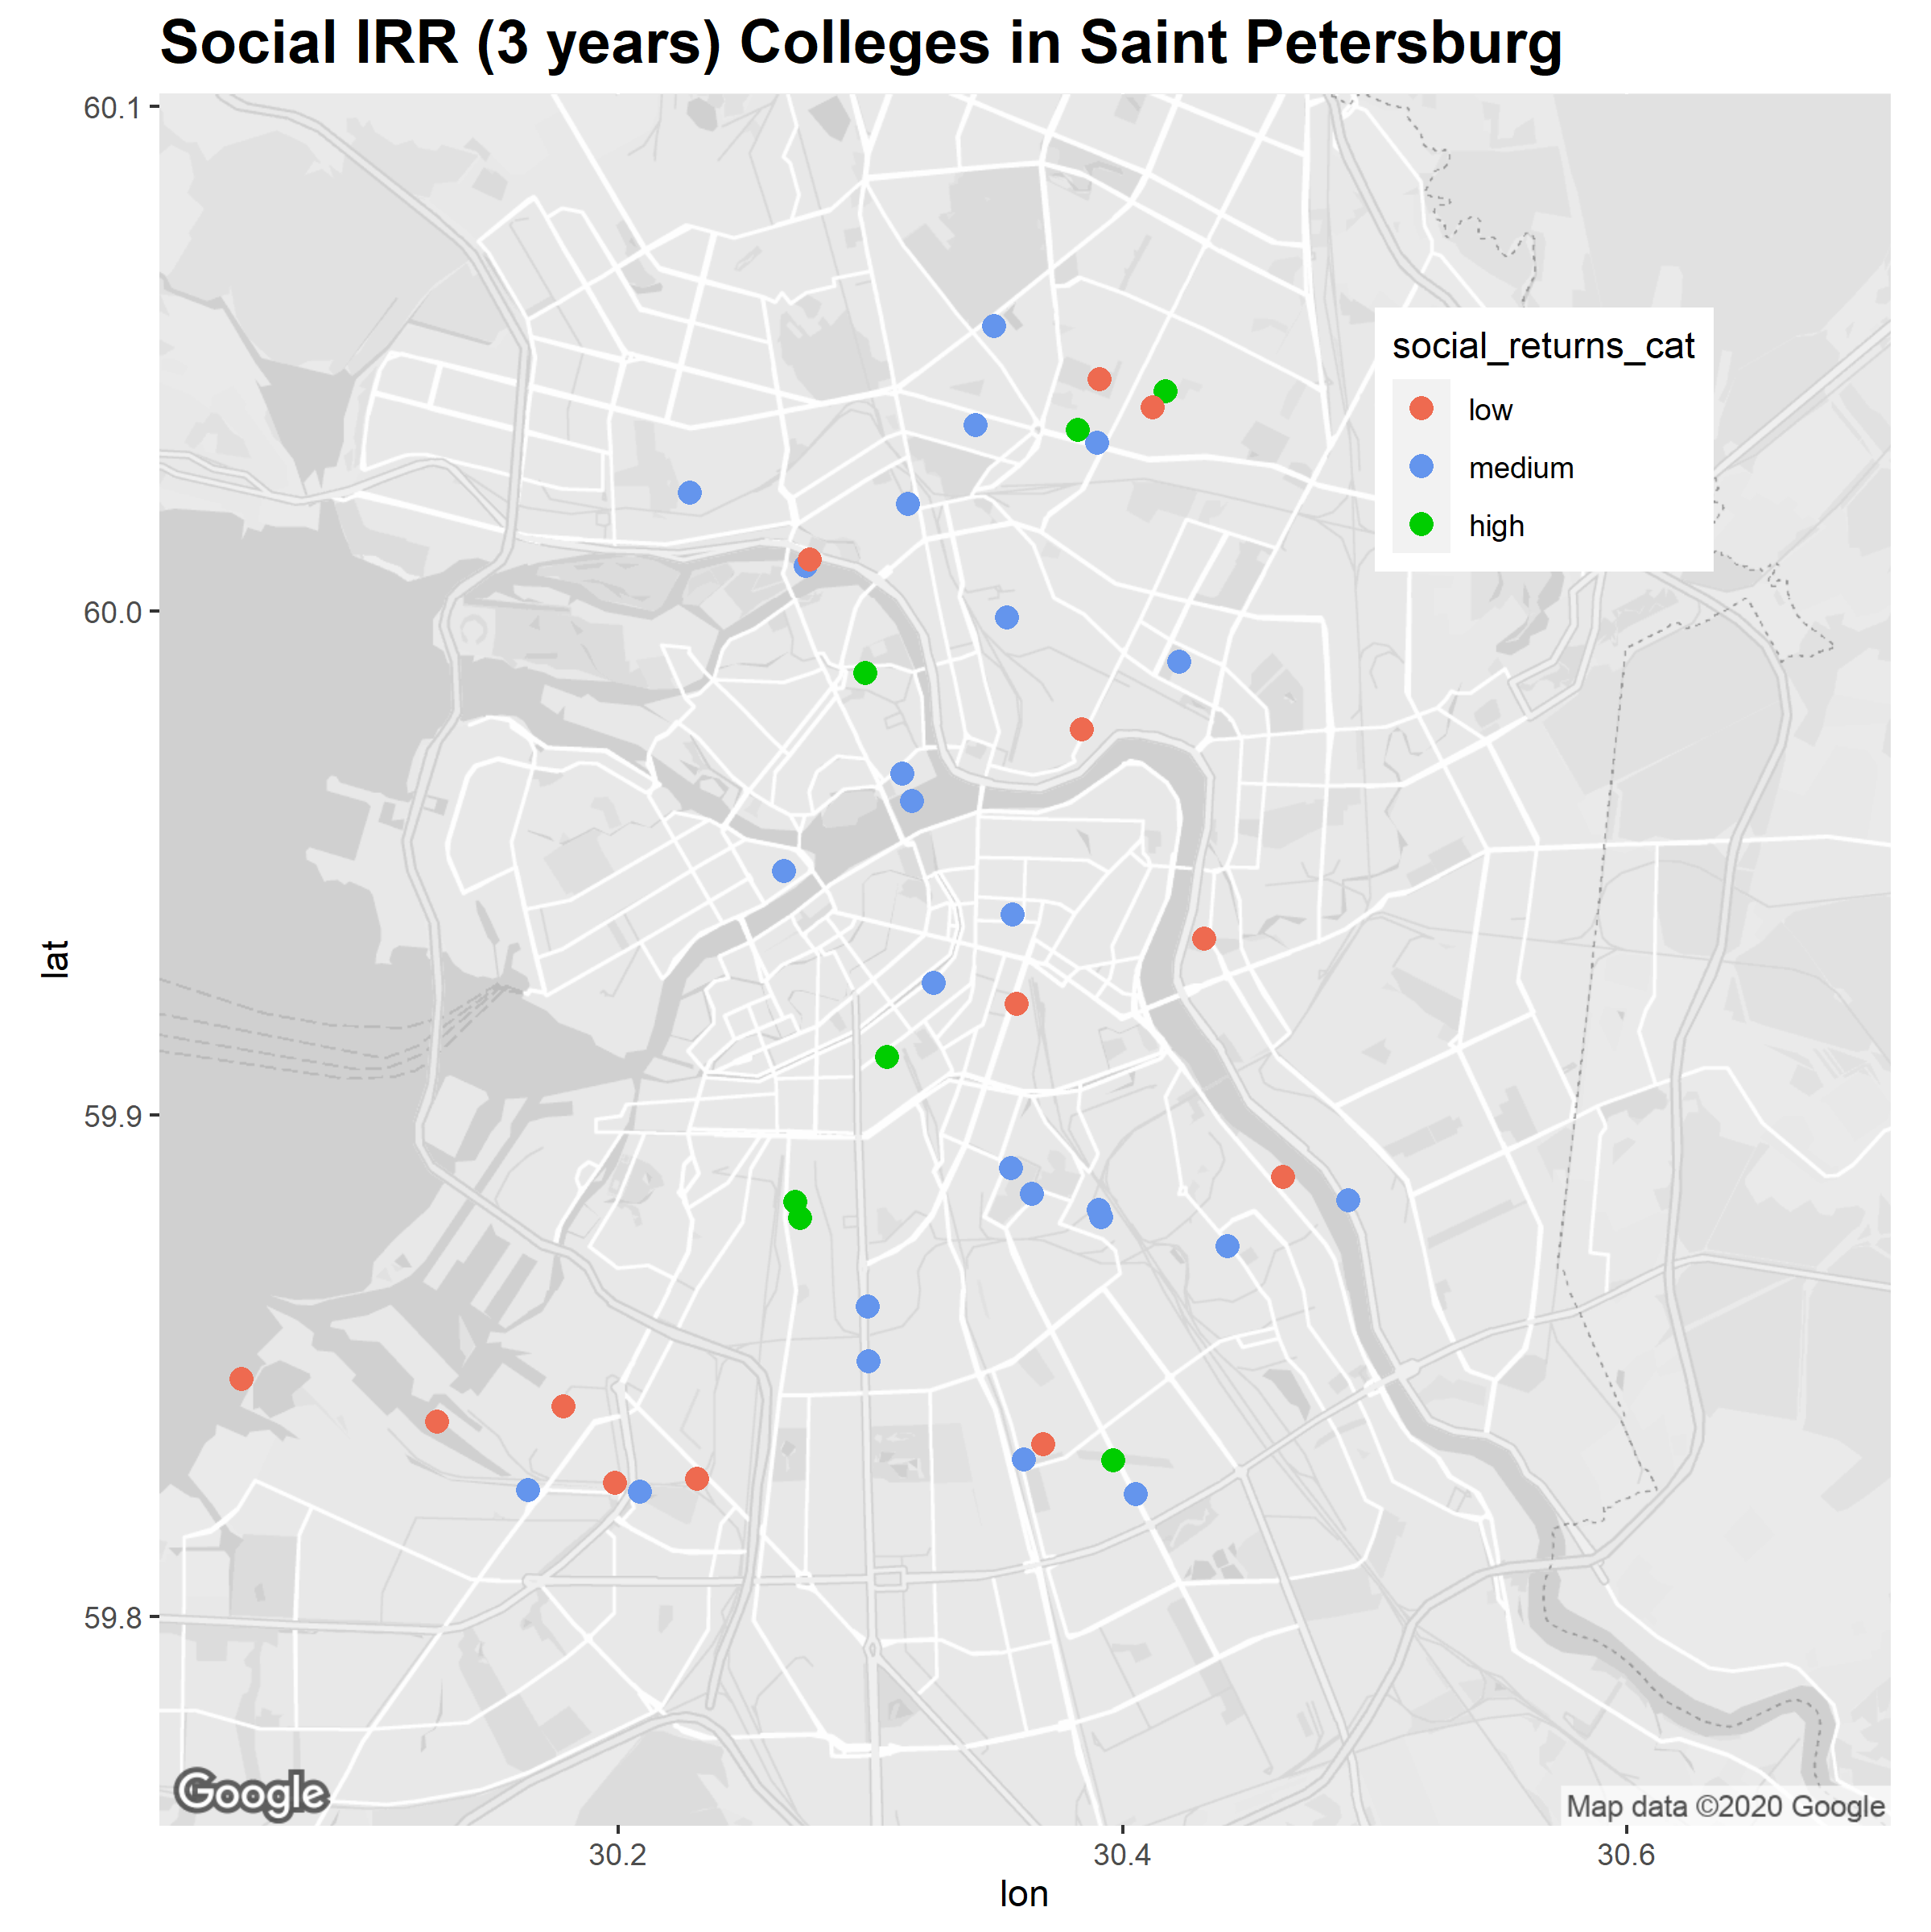
\includegraphics[width=200pt]{social_returns_spb.png}
		% plot 2
		%\subcaption{St. Petersburg}\label{}
	\end{minipage}
	\caption{Social IRR of Universities in Moscow and St. Petersburg}\label{fig:1.17}
\end{figure}




\vspace{-0.2in}

\begin{center}
	\begin{figure}[htbp!]
\begin{minipage}[b]{1\linewidth}
			\centering
			%\hspace*{-0.7in}
			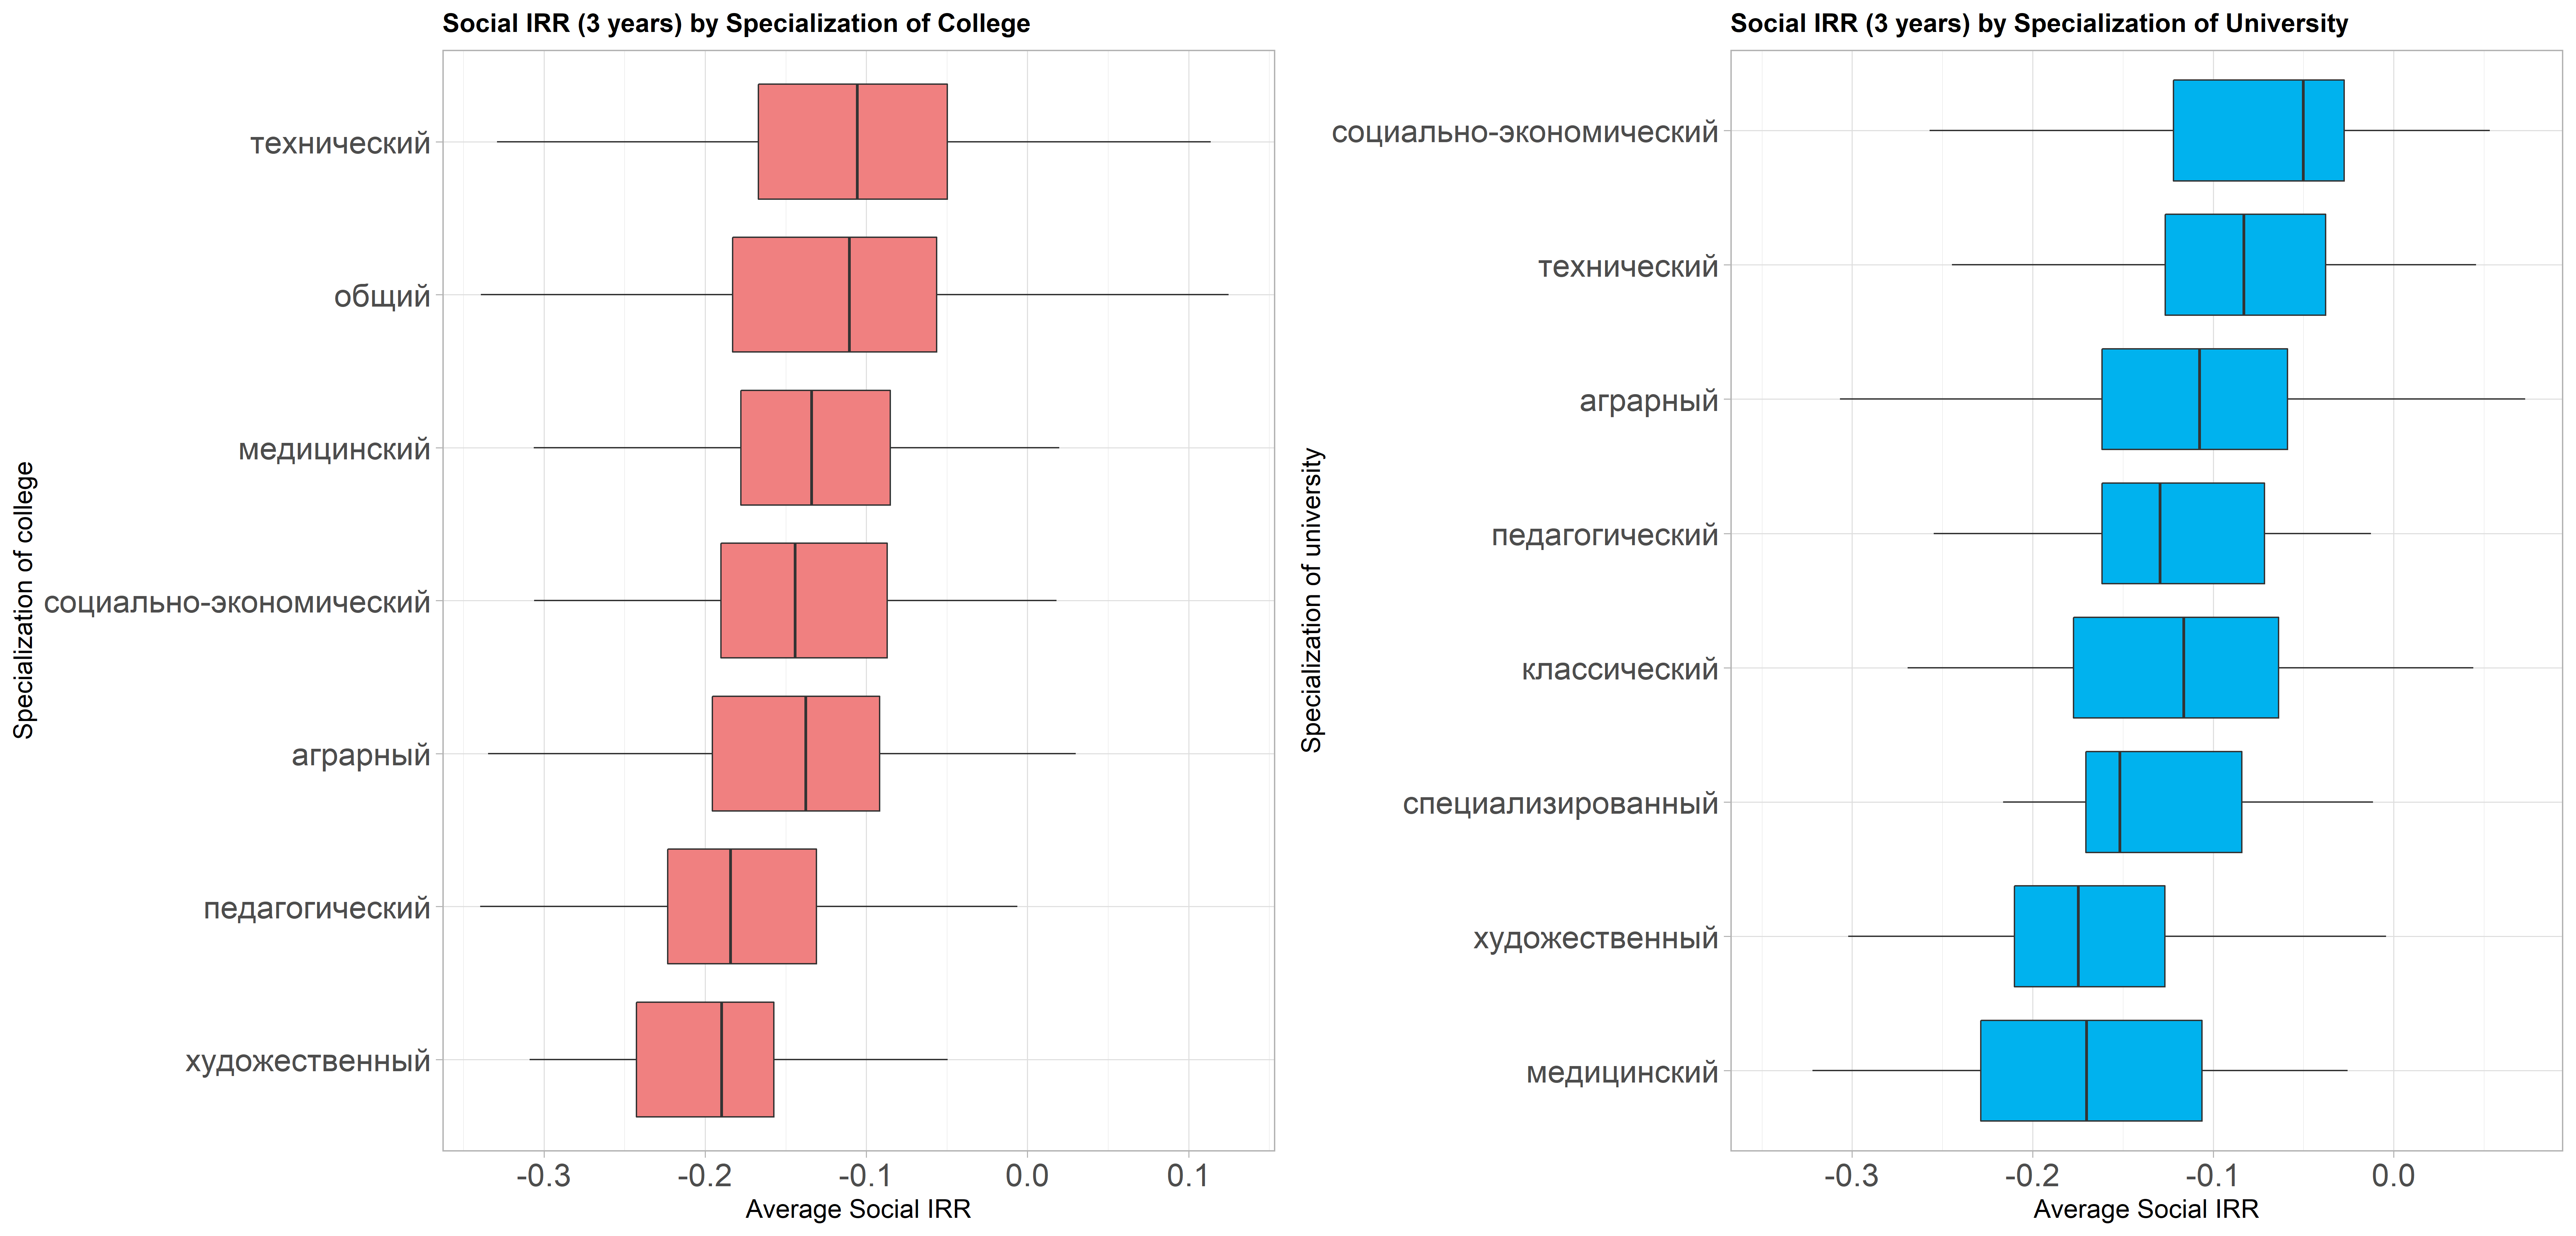
\includegraphics[width=6in]{returns_by_areas.png}
			% plot 1
		\end{minipage}
			\caption{Salary of Univ Graduates 2014 to 2016}\label{fig:1.18}
	\end{figure}
\end{center}


\newpage

\printbibliography

\newpage
\section*{Appendix}
\addcontentsline{toc}{section}{Appendix}%

\setcounter{table}{0}
\renewcommand{\thetable}{A\arabic{table}}

\setcounter{figure}{0}
\renewcommand{\thefigure}{A\arabic{figure}}


\hspace{-1in}
\fontsize{9}{11}{
	\selectfont
	\setlength{\tabcolsep}{2pt}
	\begin{longtable}{lcccccc}
		\caption{Mincerian, Private and Social Returns by Region}
		\label{tab:4.1}\\
&   \multicolumn{2}{c}{\textbf{Mincerian }} & \multicolumn{2}{c}{\textbf{Private}} & \multicolumn{2}{c}{\textbf{Social}} \\ 
	    \hline
Regions & Vocational & University & Vocational & University & Vocational & University  \\
		\hline
		\endhead
Altayskiy Kray  & $\phantom{0}\phantom{-}35.6117$ & $104.28$ & $25.77$ & $29.18$ & $18.713$ & $22.82$ \\
Amurskaya Oblast  & $\phantom{0}\phantom{-}54.6300$ & $135.14$ & $36.72$ & $34.14$ & $27.068$ & $25.86$ \\
Arkhangelskaya Oblast  & $\phantom{0}\phantom{-}86.6825$ & $186.32$ & $35.00$ & $31.52$ & $23.407$ & $23.45$ \\
Astrakhanskaya Oblast  & $\phantom{-}123.0480$ & $228.68$ & $20.45$ & $21.01$ & $18.403$ & $17.72$ \\
Bryanskaya Oblast  & $\phantom{0}\phantom{-}31.4061$ & $\phantom{0}76.75$ & $31.26$ & $34.57$ & $23.259$ & $25.88$ \\
Chechenskaya Respublika  & $\phantom{00}\phantom{-}8.5306$ & $\phantom{0}15.07$ & $27.98$ & $28.32$ & $23.022$ & $22.41$ \\
Chelyabinskaya Oblast  & $\phantom{0}\phantom{-}25.8489$ & $\phantom{0}82.98$ & $16.11$ & $18.86$ & $13.719$ & $15.72$ \\
Chukotskiy Aok  & $\phantom{0}\phantom{-}22.4758$ & $\phantom{0}55.16$ & $44.52$ & $\phantom{000}NA$ & $\phantom{0}9.742$ & $\phantom{000}NA$ \\
Chuvashskaya Respublika  & $\phantom{0}\phantom{-}31.5513$ & $102.20$ & $26.83$ & $26.24$ & $19.515$ & $22.32$ \\
Evreyskaya AOb  & $\phantom{0}\phantom{-}36.1407$ & $109.63$ & $31.46$ & $33.91$ & $19.195$ & $24.42$ \\
Irkutskaya Oblast  & $\phantom{0}\phantom{-}39.1235$ & $129.45$ & $28.55$ & $36.67$ & $19.941$ & $28.63$ \\
Ivanovskaya Oblast  & $\phantom{0}\phantom{-}16.0425$ & $\phantom{0}56.23$ & $32.93$ & $40.47$ & $20.984$ & $21.28$ \\
Kaliningradskaya Oblast  & $\phantom{0}\phantom{-}20.3191$ & $\phantom{0}57.20$ & $30.24$ & $27.05$ & $20.869$ & $21.97$ \\
Kaluzhskaya Oblast  & $\phantom{0}\phantom{-}19.2983$ & $\phantom{0}62.37$ & $20.89$ & $23.41$ & $15.925$ & $21.20$ \\
Kamchatskaya Kray  & $\phantom{0}\phantom{-}35.8895$ & $106.29$ & $39.26$ & $44.74$ & $21.232$ & $34.86$ \\
Kemerovskaya Oblast  & $\phantom{0}\phantom{-}28.0464$ & $\phantom{0}76.21$ & $40.00$ & $29.93$ & $24.212$ & $23.27$ \\
Khabarovskiy Kray  & $\phantom{0}\phantom{-}59.8920$ & $153.14$ & $32.52$ & $37.88$ & $21.508$ & $29.75$ \\
Khanty-Mansiyskiy Aok  & $\phantom{0}\phantom{-}50.1452$ & $118.32$ & $54.37$ & $51.20$ & $23.741$ & $28.96$ \\
Kirovskaya Oblast  & $\phantom{00}\phantom{-}9.2090$ & $\phantom{0}81.50$ & $29.35$ & $24.18$ & $20.630$ & $19.49$ \\
Kostromskaya Oblast  & $\phantom{0}\phantom{-}42.6683$ & $107.65$ & $17.96$ & $19.72$ & $15.363$ & $17.14$ \\
Krasnodarskiy Kray  & $\phantom{00}\phantom{-}9.2547$ & $\phantom{0}94.33$ & $30.48$ & $29.40$ & $21.451$ & $24.33$ \\
Krasnoyarskiy Kray  & $\phantom{0}\phantom{-}28.2208$ & $\phantom{0}63.64$ & $42.31$ & $35.53$ & $25.562$ & $23.30$ \\
Kurganskaya Oblast  & $\phantom{0}\phantom{-}23.6786$ & $119.31$ & $15.28$ & $14.24$ & $11.714$ & $13.53$ \\
Kurskaya Oblast  & $\phantom{0}\phantom{-}43.1486$ & $\phantom{0}93.43$ & $21.86$ & $17.99$ & $17.055$ & $16.17$ \\
Leningradskaya Oblast  & $\phantom{0}\phantom{-}58.2302$ & $100.19$ & $30.34$ & $32.65$ & $18.887$ & $27.82$ \\
Lipetskaya Oblast  & $\phantom{0}\phantom{-}41.6088$ & $107.96$ & $30.69$ & $29.98$ & $23.169$ & $24.46$ \\
Moscow  & $\phantom{00}\phantom{-}9.5503$ & $\phantom{0}55.65$ & $32.59$ & $34.86$ & $20.193$ & $24.76$ \\
Murmanskaya Oblast  & $\phantom{0}\phantom{-}30.5068$ & $107.80$ & $32.83$ & $36.61$ & $21.522$ & $28.64$ \\
Nenetskiy Aok  & $\phantom{0}\phantom{-}88.3374$ & $175.64$ & $57.12$ & $\phantom{000}NA$ & $18.737$ & $\phantom{000}NA$ \\
Nizhegorodskaya Oblast  & $\phantom{0}\phantom{-}18.1549$ & $\phantom{0}85.31$ & $45.19$ & $38.53$ & $25.478$ & $29.55$ \\
Novgorodskaya Oblast  & $\phantom{0}\phantom{-}20.5742$ & $\phantom{0}66.75$ & $32.94$ & $33.85$ & $25.034$ & $26.07$ \\
Novosibirskaya Oblast  & $\phantom{0}\phantom{-}75.2078$ & $137.75$ & $44.75$ & $36.63$ & $29.225$ & $27.67$ \\
Omskaya Oblast  & $\phantom{0}\phantom{-}36.7901$ & $\phantom{0}64.86$ & $28.54$ & $23.70$ & $19.238$ & $19.29$ \\
Orenburgskaya Oblast  & $\phantom{0}\phantom{-}47.3624$ & $\phantom{0}97.24$ & $28.75$ & $28.99$ & $22.446$ & $23.51$ \\
Orlovskaya Oblast  & $\phantom{0}\phantom{-}16.9054$ & $\phantom{0}70.80$ & $29.46$ & $31.55$ & $22.305$ & $23.43$ \\
Penzenskaya Oblast  & $\phantom{00}\phantom{-}5.4499$ & $\phantom{0}19.22$ & $37.20$ & $35.71$ & $25.621$ & $30.65$ \\
Permskiy Krai  & $\phantom{0}\phantom{-}47.4043$ & $104.89$ & $34.55$ & $32.45$ & $26.654$ & $26.69$ \\
Primorskiy Kray  & $\phantom{0}\phantom{-}26.8830$ & $104.89$ & $41.39$ & $37.60$ & $33.279$ & $24.48$ \\
Pskovskaya Oblast  & $\phantom{0}\phantom{-}19.1578$ & $\phantom{0}72.85$ & $31.53$ & $25.48$ & $23.623$ & $20.84$ \\
Respublika Adygeya  & $\phantom{0}\phantom{-}21.1613$ & $\phantom{0}40.15$ & $32.22$ & $35.76$ & $23.017$ & $25.87$ \\
Respublika Altay  & $\phantom{0}\phantom{-}47.3321$ & $202.43$ & $20.45$ & $29.13$ & $10.785$ & $22.56$ \\
Respublika Buryatia  & $\phantom{0}\phantom{-}32.7424$ & $\phantom{0}55.87$ & $37.60$ & $33.10$ & $23.601$ & $27.50$ \\
Respublika Kalmykiya  & $\phantom{0}\phantom{-}53.7437$ & $127.49$ & $19.91$ & $\phantom{000}NA$ & $15.754$ & $\phantom{000}NA$ \\
Respublika Karelia  & $\phantom{0}\phantom{-}17.7606$ & $\phantom{0}42.27$ & $32.91$ & $30.49$ & $23.299$ & $20.83$ \\
Respublika Khakasiya  & $\phantom{0}\phantom{-}47.3759$ & $125.62$ & $28.60$ & $31.15$ & $19.527$ & $24.72$ \\
Respublika Komi  & $\phantom{0}\phantom{-}42.3682$ & $115.35$ & $43.55$ & $36.78$ & $26.769$ & $31.00$ \\
Respublika Mariy El  & $\phantom{0}\phantom{-}20.6738$ & $\phantom{0}73.38$ & $31.53$ & $28.72$ & $23.151$ & $22.65$ \\
Respublika Mordovia  & $\phantom{0}\phantom{-}18.6844$ & $\phantom{0}51.72$ & $15.87$ & $18.50$ & $13.186$ & $15.58$ \\
Respublika Saha (Yakutia)  & $\phantom{0}\phantom{-}31.0007$ & $\phantom{0}95.71$ & $37.58$ & $42.78$ & $22.142$ & $27.40$ \\
Respublika Severnaya Osetiya  & $\phantom{00}-4.6462$ & $\phantom{0}38.53$ & $42.56$ & $34.57$ & $30.019$ & $26.41$ \\
Respublika Tatarstan  & $\phantom{0}\phantom{-}42.6535$ & $100.88$ & $32.50$ & $28.06$ & $26.922$ & $22.20$ \\
Rostovskaya Oblast  & $\phantom{0}\phantom{-}54.8784$ & $131.19$ & $34.24$ & $31.47$ & $23.995$ & $20.25$ \\
Ryazanskaya Oblast  & $\phantom{0}\phantom{-}18.9791$ & $\phantom{0}90.79$ & $34.81$ & $29.92$ & $25.270$ & $24.81$ \\
Saint-Petersburg  & $\phantom{00}\phantom{-}0.8399$ & $\phantom{0}38.48$ & $44.68$ & $40.00$ & $22.098$ & $28.01$ \\
Sakhalinskaya Oblast  & $\phantom{0}\phantom{-}33.2860$ & $176.91$ & $35.62$ & $44.33$ & $17.853$ & $31.94$ \\
Samarskaya Oblast  & $\phantom{0}\phantom{-}40.4262$ & $115.60$ & $36.93$ & $37.40$ & $26.895$ & $28.82$ \\
Smolenskaya Oblast  & $\phantom{0}\phantom{-}18.5241$ & $\phantom{0}85.55$ & $27.01$ & $18.00$ & $20.954$ & $18.15$ \\
Stavropolskiy Kray  & $\phantom{0}\phantom{-}16.4360$ & $\phantom{0}90.99$ & $27.72$ & $27.73$ & $23.933$ & $23.44$ \\
Sverdlovskaya Oblast  & $\phantom{0}\phantom{-}47.3084$ & $137.55$ & $32.74$ & $33.17$ & $22.039$ & $23.60$ \\
Tambovskaya Oblast  & $\phantom{00}\phantom{-}2.5801$ & $\phantom{0}42.60$ & $32.74$ & $45.09$ & $21.456$ & $37.41$ \\
Tomskaya Oblast  & $\phantom{0}\phantom{-}63.9402$ & $175.02$ & $26.96$ & $27.34$ & $20.205$ & $19.20$ \\
Tulskaya Oblast  & $\phantom{0}\phantom{-}34.3715$ & $\phantom{0}80.53$ & $36.90$ & $36.40$ & $24.753$ & $28.54$ \\
Tverskaya Oblast  & $\phantom{00}\phantom{-}5.0335$ & $\phantom{0}46.01$ & $32.76$ & $27.27$ & $23.193$ & $22.60$ \\
Tyumenskaya Oblast  & $\phantom{-}142.9216$ & $244.89$ & $27.58$ & $20.22$ & $18.337$ & $18.56$ \\
Ul'yanovskaya Oblast  & $\phantom{0}\phantom{-}50.6008$ & $\phantom{0}97.46$ & $30.36$ & $47.52$ & $24.978$ & $39.53$ \\
Vladimirskaya Oblast  & $\phantom{00}\phantom{-}8.4301$ & $\phantom{0}58.59$ & $37.42$ & $45.47$ & $23.893$ & $34.26$ \\
Volgogradskaya Oblast  & $\phantom{0}\phantom{-}58.1734$ & $115.78$ & $28.06$ & $23.50$ & $21.873$ & $18.42$ \\
Vologodskaya Oblast  & $\phantom{0}\phantom{-}42.0563$ & $148.48$ & $36.11$ & $37.62$ & $27.850$ & $31.95$ \\
Voronezhskaya Oblast  & $\phantom{0}\phantom{-}14.9261$ & $\phantom{0}72.07$ & $30.06$ & $27.75$ & $22.511$ & $23.00$ \\
Yaroslavskaya Oblast  & $\phantom{0}\phantom{-}32.1941$ & $142.41$ & $31.83$ & $35.69$ & $21.751$ & $28.06$ \\
		\hline 
	\end{longtable}
 
}
 

\begin{center}
	\begin{figure}[htbp!]
\begin{minipage}[b]{1\linewidth}
			\centering
			%\hspace*{-0.7in}
			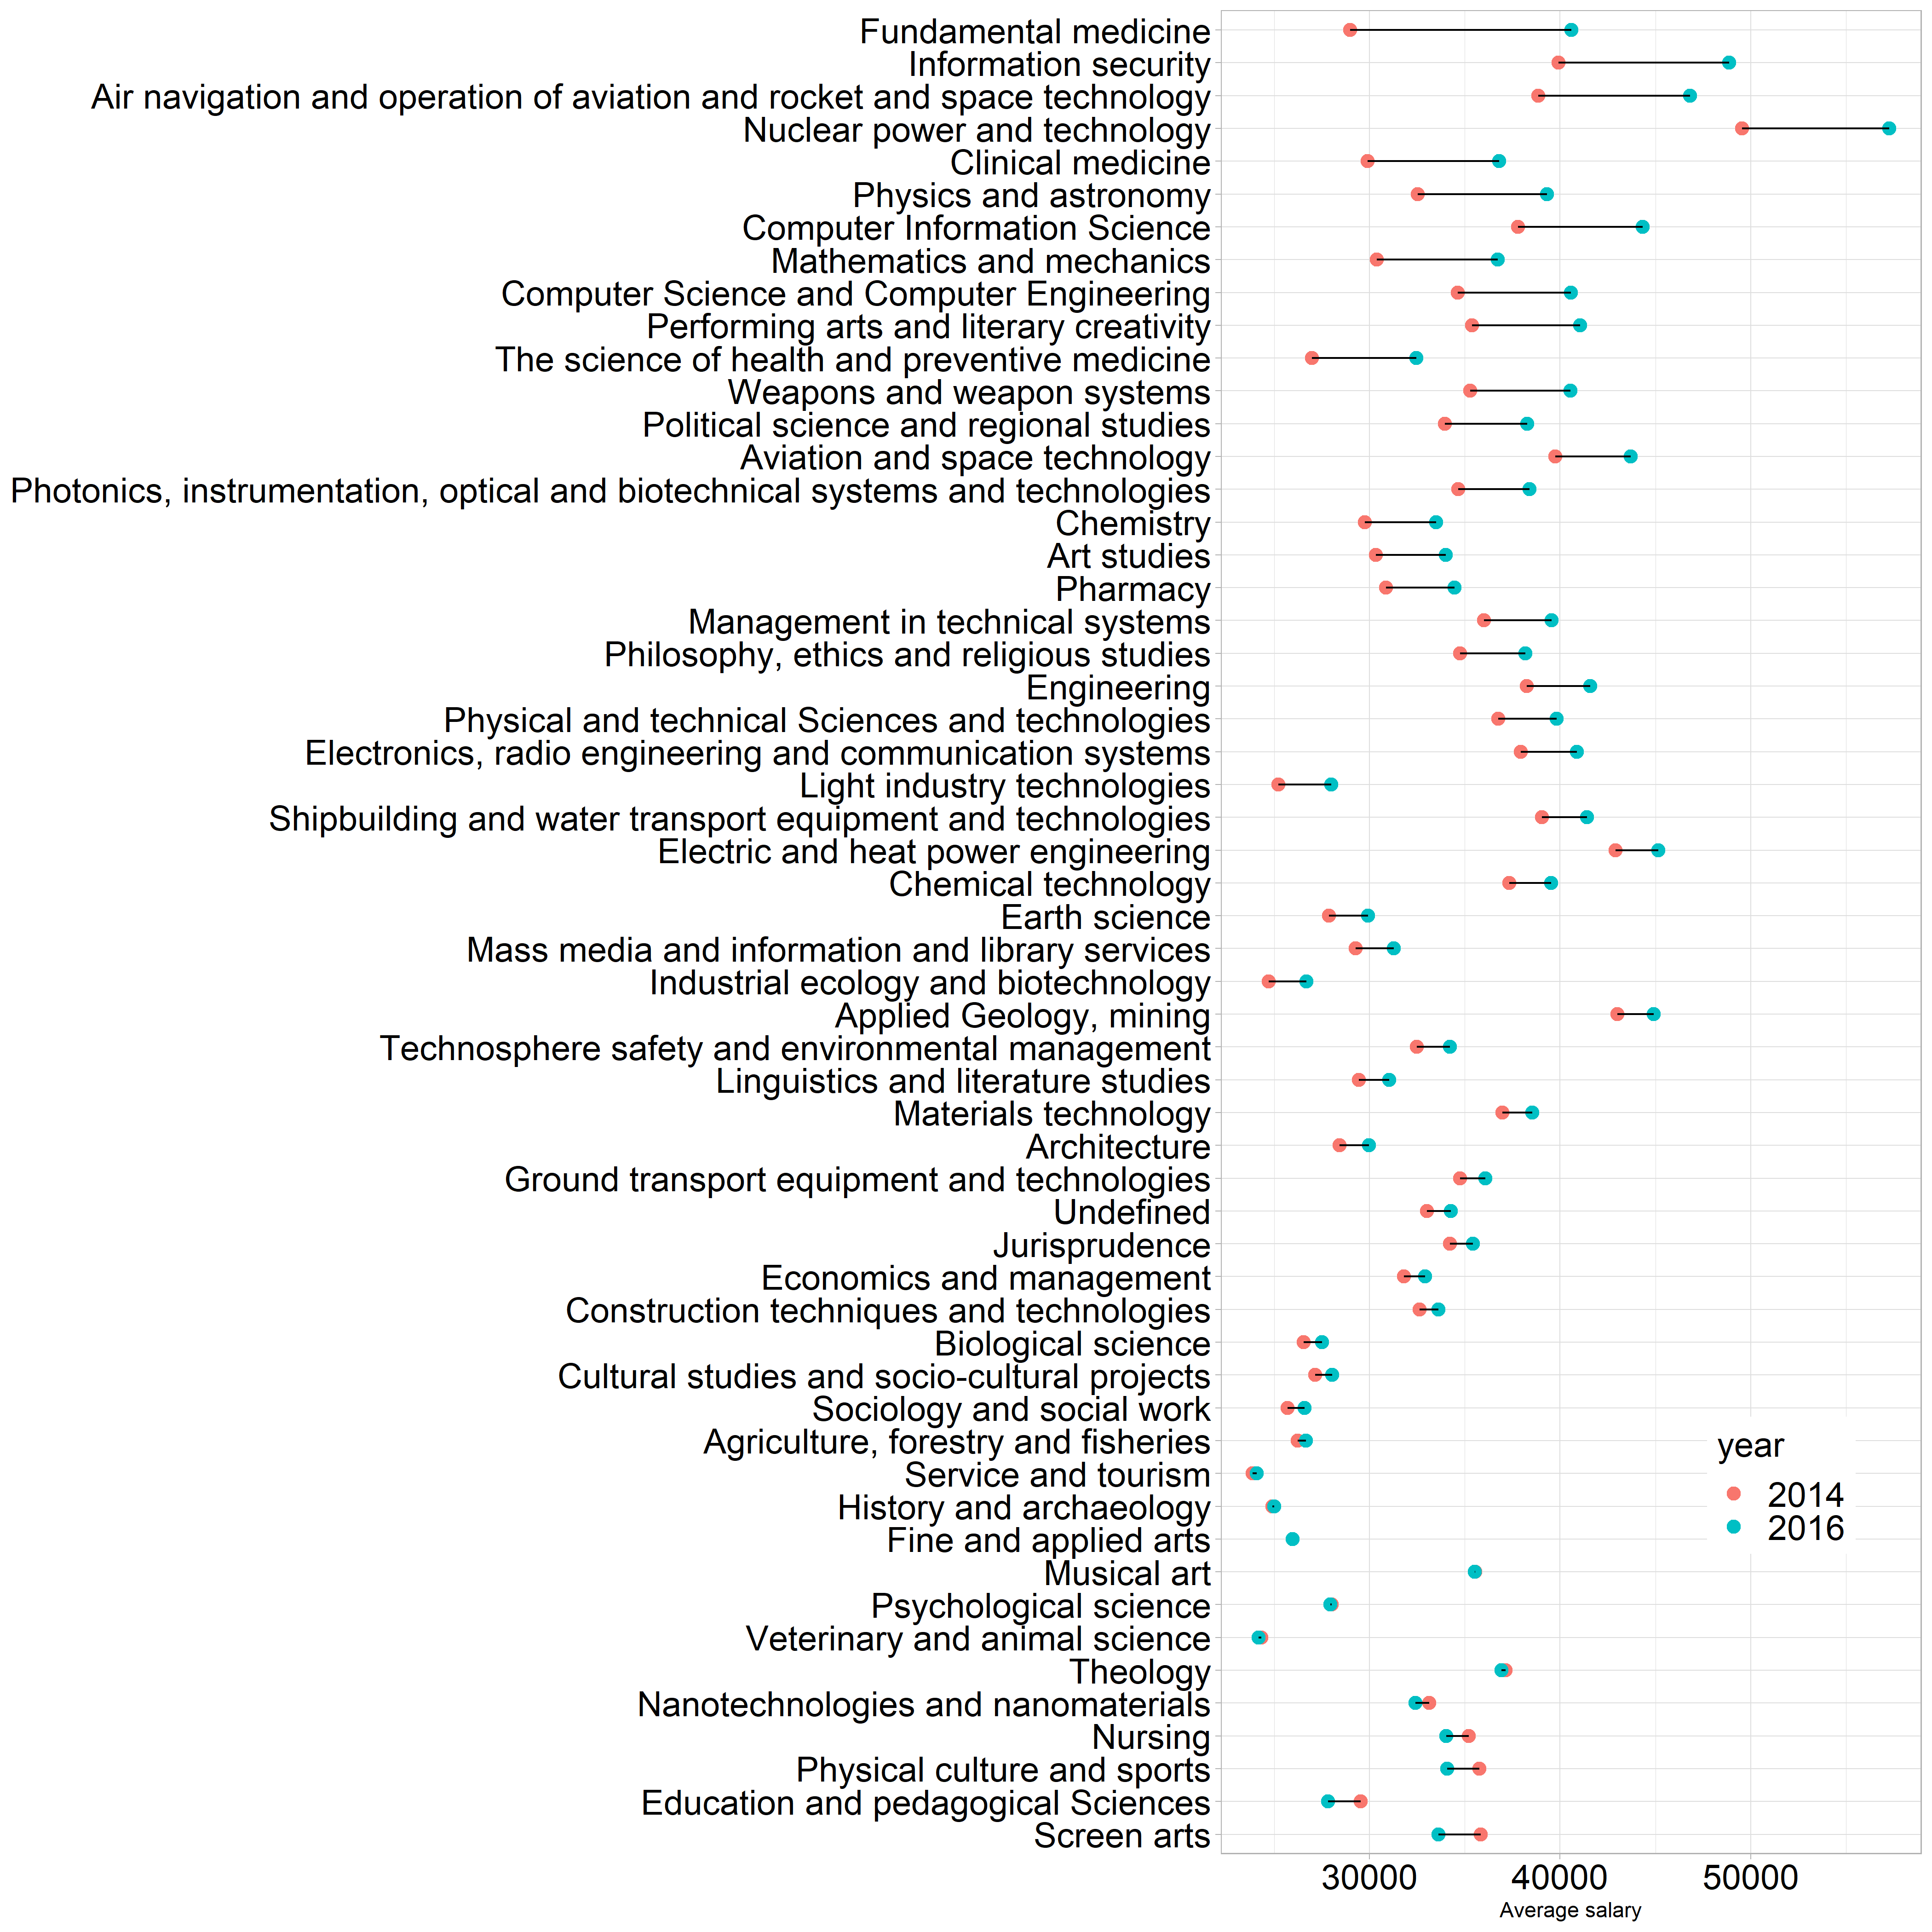
\includegraphics[width=6in]{sal_area.png}
			% plot 1
		\end{minipage}
			\caption{Salary of Univ Graduates 2014 to 2016}\label{fig:7.6}
	\end{figure}
\end{center}



\end{document}
